\documentclass{article}

% if you need to pass options to natbib, use, e.g.:
%     \PassOptionsToPackage{numbers, compress}{natbib}
% before loading neurips_2026

% The authors should use one of these tracks.
% Before accepting by the NeurIPS conference, select one of the options below.
% 0. "default" for submission
\usepackage{neurips_2026}
% the "default" option is equal to the "main" option, which is used for the Main Track with double-blind reviewing.
% 1. "main" option is used for the Main Track
%  \usepackage[main]{neurips_2026}
% 2. "position" option is used for the Position Paper Track
%  \usepackage[position]{neurips_2026}
% 3. "eandd" option is used for the Evaluations & Datasets Track
 % \usepackage[eandd]{neurips_2026}
% 4. "creativeai" option is used for the Creative AI Track
%  \usepackage[creativeai]{neurips_2026}
% 5. "sglblindworkshop" option is used for the Workshop with single-blind reviewing
 % \usepackage[sglblindworkshop]{neurips_2026}
% 6. "dblblindworkshop" option is used for the Workshop with double-blind reviewing
%  \usepackage[dblblindworkshop]{neurips_2026}

% After being accepted, the authors should add "final" behind the track to compile a camera-ready version.
% 1. Main Track
 % \usepackage[main, final]{neurips_2026}
% 2. Position Paper Track
%  \usepackage[position, final]{neurips_2026}
% 3. Evaluations & Datasets Track
 % \usepackage[eandd, final]{neurips_2026}
% 4. Creative AI Track
%  \usepackage[creativeai, final]{neurips_2026}
% 5. Workshop with single-blind reviewing
%  \usepackage[sglblindworkshop, final]{neurips_2026}
% 6. Workshop with double-blind reviewing
%  \usepackage[dblblindworkshop, final]{neurips_2026}
% Note. For the workshop paper template, both \title{} and \workshoptitle{} are required, with the former indicating the paper title shown in the title and the latter indicating the workshop title displayed in the footnote.
% For workshops (5., 6.), the authors should add the name of the workshop, "\workshoptitle" command is used to set the workshop title.
% \workshoptitle{WORKSHOP TITLE}

% "preprint" option is used for arXiv or other preprint submissions
 % \usepackage[preprint]{neurips_2026}

% to avoid loading the natbib package, add option nonatbib:
%    \usepackage[nonatbib]{neurips_2026}

\usepackage[utf8]{inputenc} % allow utf-8 input
\usepackage[T1]{fontenc}    % use 8-bit T1 fonts
\usepackage{hyperref}       % hyperlinks
\usepackage{url}            % simple URL typesetting
\usepackage{booktabs}       % professional-quality tables
\usepackage{amsfonts}       % blackboard math symbols
\usepackage{nicefrac}       % compact symbols for 1/2, etc.
\usepackage{microtype}      % microtypography
\usepackage{xcolor}         % colors

\usepackage{amsmath}
\usepackage{amssymb}
\usepackage{amsthm}
\usepackage{graphicx}
\usepackage{tikz}
\usetikzlibrary{arrows.meta}
\usepackage{algorithm}
\usepackage{algorithmic}
\usepackage{multirow}
\usepackage{subcaption}
\usepackage{wrapfig}
\usepackage{pifont}
\usepackage{afterpage}

\definecolor{citecolor}{HTML}{0066CC}
\hypersetup{colorlinks=true, linkcolor=citecolor, citecolor=citecolor, urlcolor=citecolor}
\newcommand{\sketch}{\textsc{Sketch}}
\newcommand{\ccv}{\textsc{CCV}}
\newcommand{\kgated}{$\kappa$-gated}
\newcommand{\pp}{\,\text{pp}}
\newcommand{\recheck}[1]{\textcolor{red}{#1}}

\newtheorem{proposition}{Proposition}
\newtheorem{theorem}{Theorem}
\newtheorem{lemma}{Lemma}
\newtheorem{definition}{Definition}
\newtheorem{corollary}{Corollary}

\title{Cross-Channel Agreement Beats Consensus: Compositional Verification for Geometry Reasoning}

\author{
  Anonymous Authors
}

\begin{document}

\maketitle

% ===========================================================================
\begin{abstract}
% User-supplied abstract retained verbatim apart from TeX typography and red aggregate markers.
% AUTHOR CHECK: its independence, four-benchmark, inference-cost, and domain-scope wording
% conflicts with the revised body; see task/revision_notes.md and checklist item 1.

Multimodal geometry reasoning requires jointly perceiving diagrams and performing symbolic derivations. Test-time verification methods such as majority voting assume voter errors are roughly independent, but in geometry all candidates perceive the same diagram, so perceptual biases cascade into correlated errors that produce confident but wrong consensus---repeating a vote within one channel cannot escape a shared misperception. To expose a structurally independent signal, we standardize each candidate into SKETCH, a format that decomposes reasoning into a neural pathway (natural-language claim) and a symbolic pathway (visual grounding $\rightarrow$ typed program $\rightarrow$ deterministic execution). Because these two pathways fail through different error processes, their agreement carries information that within-channel repetition cannot. Compositional Consensus Verification (CCV), our training-free verifier, gates consensus on this cross-pathway agreement---a precision filter that retains only candidates whose two pathways independently converge, making each concordant vote far more reliable than a raw majority vote. Across four geometry benchmarks, CCV reaches \recheck{81.0\%} accuracy (\recheck{+10.4} pp over majority voting) with no external scorers or extra inference, and transfers to a second model family (\recheck{+7.8} pp). Seven non-compositional baselines---including trained reward models---cluster at \recheck{70--71\%}, while cross-channel methods jump to \recheck{79--81\%}, confirming that structural diversity, not more votes, is the core verification resource.

\end{abstract}

% ===========================================================================
\section{Introduction}
\label{sec:intro}
% ===========================================================================

\begin{figure}[t]
    \centering
    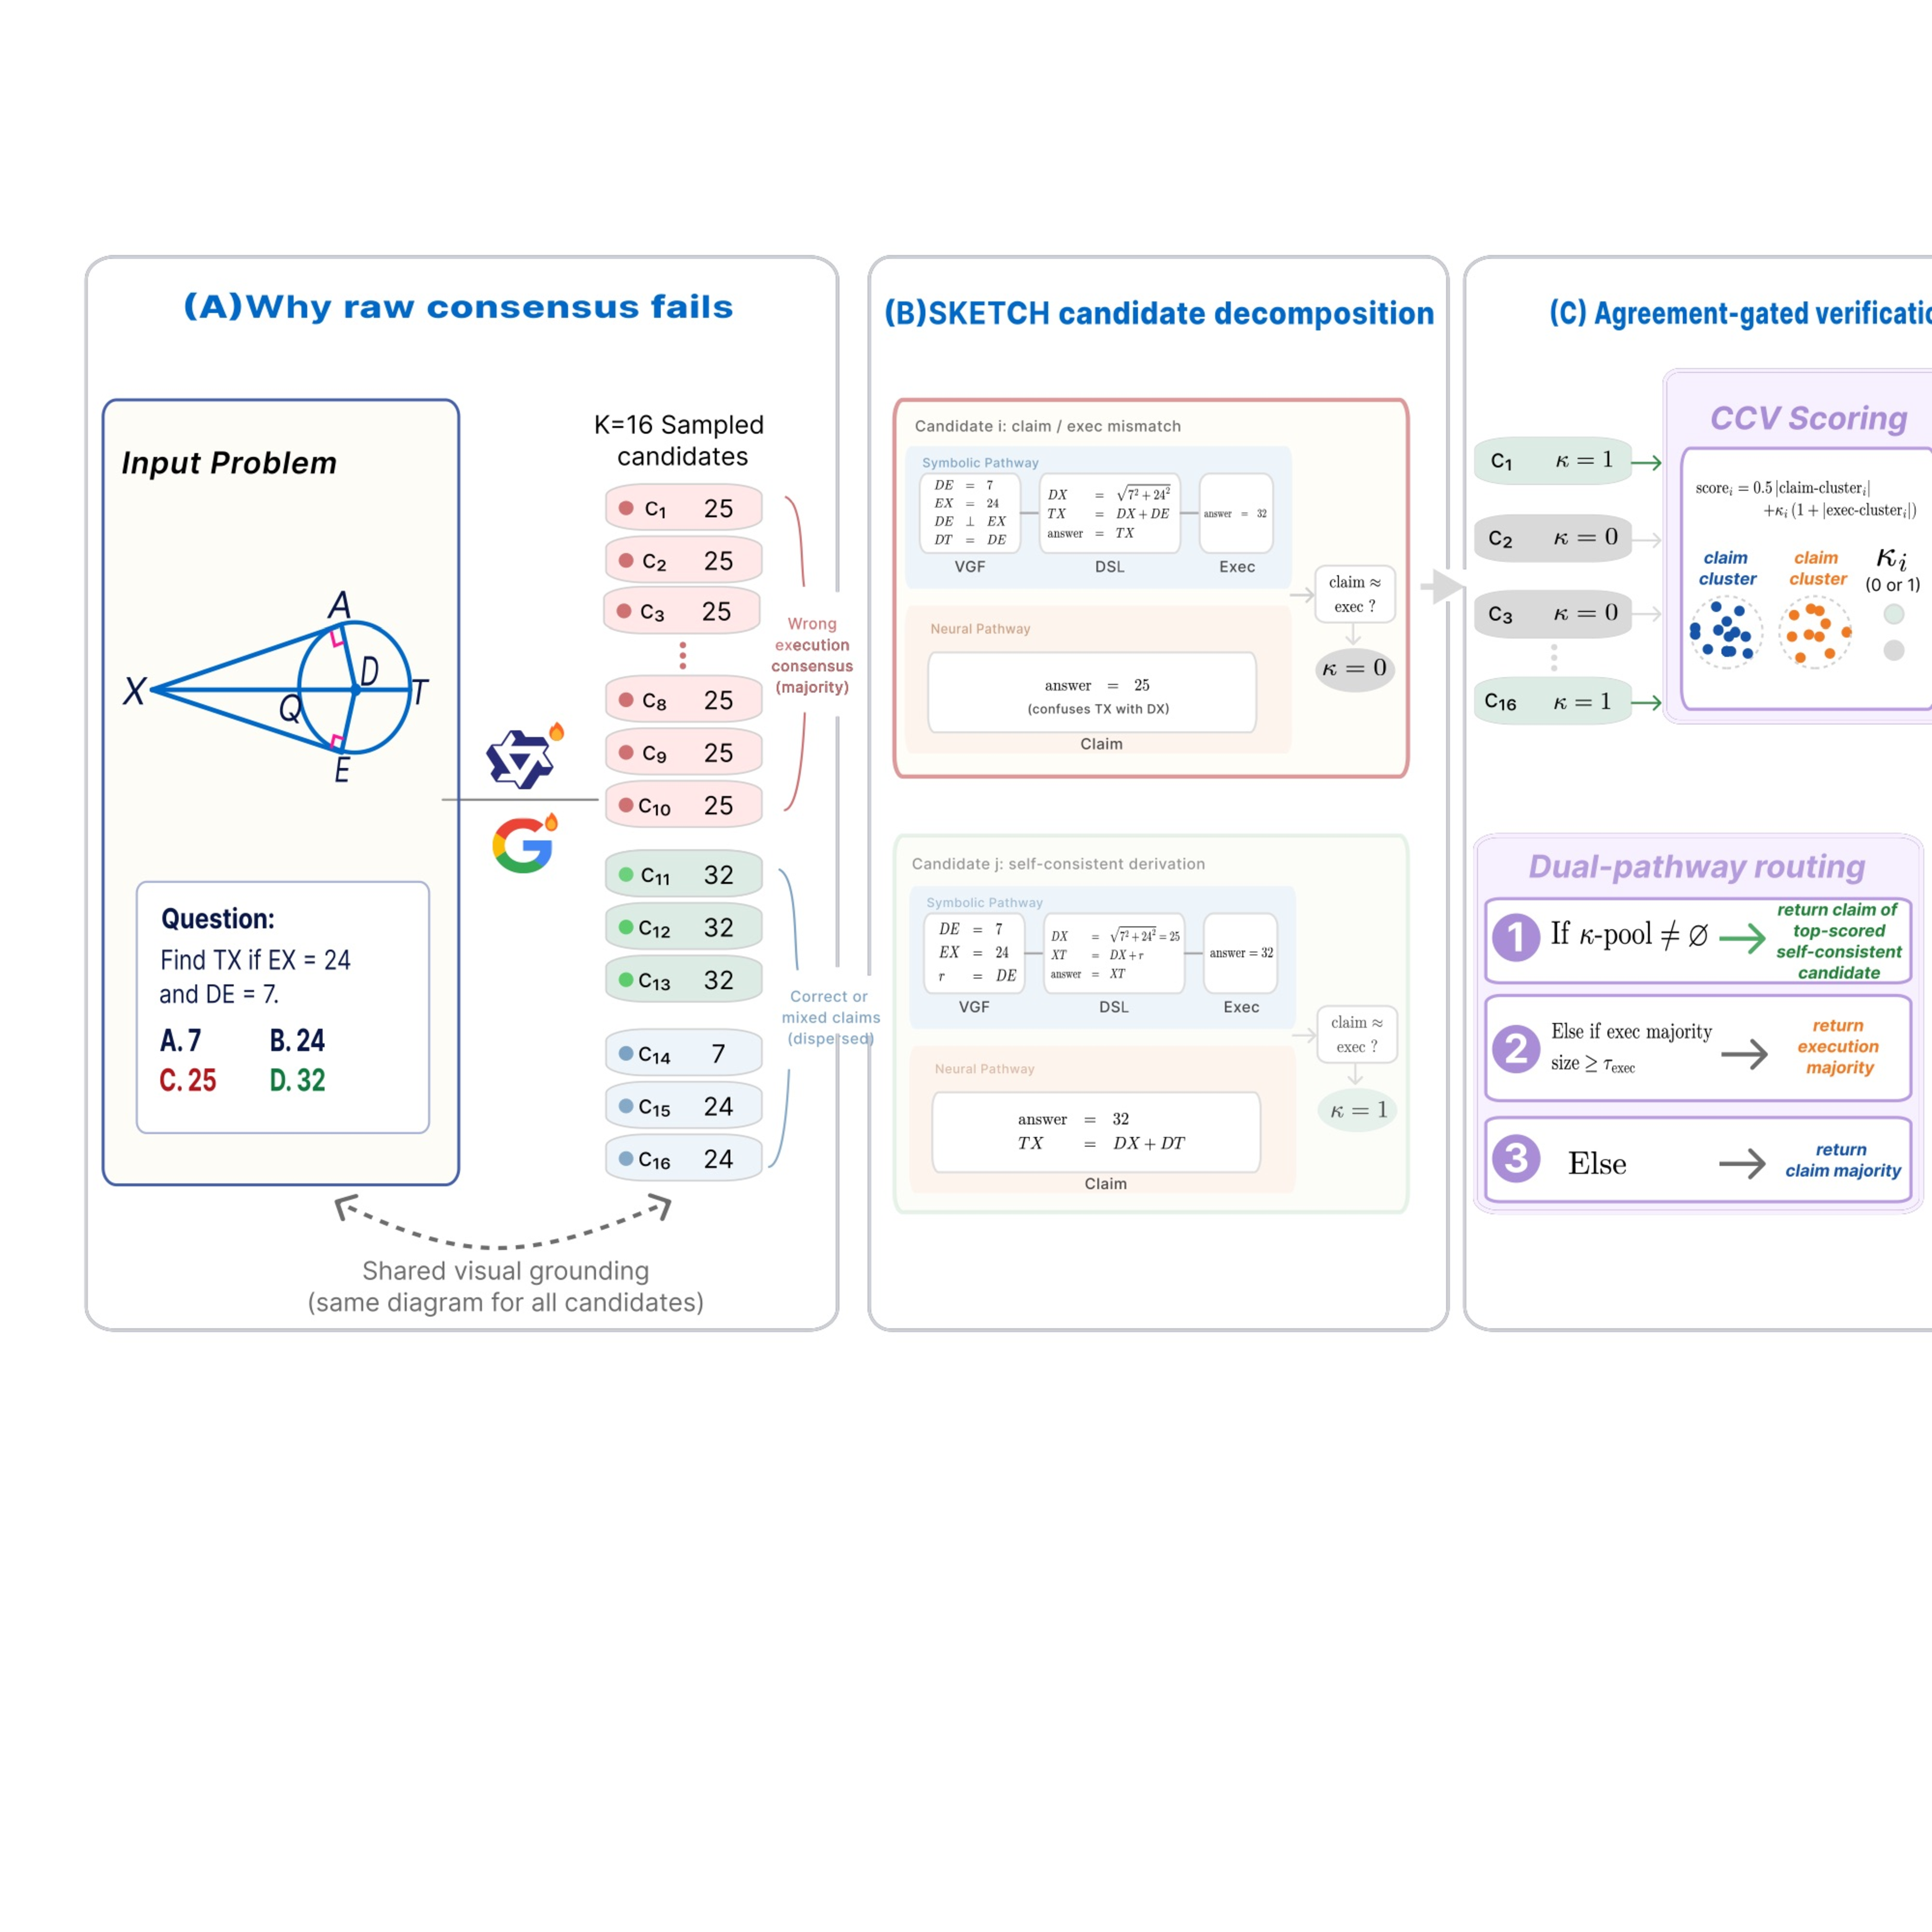
\includegraphics[width=\linewidth]{figures/figure1.pdf}
    \caption{\textbf{CCV architecture overview.} A geometry problem is processed to sample $K{=}16$ \sketch{} candidates. Each candidate exposes a symbolic reasoning pathway (visual grounding $\rightarrow$ a typed domain-specific language (DSL) $\rightarrow$ execution) and a neural intuition pathway (claim). Cross-channel agreement $\kappa$ acts as a precision filter to gate consensus; when agreement collapses, the system falls back to execution or claim majority. Execution is performed externally after generation; the claim sees the DSL source but not its executed output.}
    \label{fig:method-overview}
\end{figure}

\paragraph{The verification bottleneck in geometry reasoning.}
Geometry reasoning differs from purely textual mathematical tasks in a fundamental way: it requires joint visual perception and symbolic derivation. A model must read spatial relationships from a diagram---angles, parallel lines, congruences---and then chain these percepts through multi-step logical deductions. This conjunction makes geometry a task that current vision-language models (VLMs) find difficult~\citep{gao2023g,xia2024geox,zhang2024mavis}, and it also creates a distinctive failure mode for test-time verification. Figure~\ref{fig:method-overview} summarizes our proposed solution.

The standard approach for improving reasoning accuracy at test time is self-consistency~\citep{wang2022self}: sample $K$ candidates and select the most frequent answer via majority voting (MV). A classical Condorcet justification assumes independent, sufficiently accurate voters, so that binary majority reliability improves as $K$ grows. In geometry, this assumption breaks down in a specific and measurable way. All $K$ candidates perceive the \emph{same} diagram; if the model harbors a systematic perceptual bias---misidentifying a perpendicular as supplementary, or misreading an angle label---then a majority of candidates will share the same error. Votes become correlated because they reflect the same perceptual errors. Formally, when the pairwise error correlation $\rho$ is substantial, the effective sample size degrades as $N_{\text{eff}} = K / (1 + (K{-}1)\rho)$~\citep{ladha1992condorcet,nitarach2026model}. At $\rho = 0.5$, sixteen candidates carry the information of barely two independent votes. In our experiments, wrong execution consensus clusters of size 8--16 account for \recheck{86\%} of the execution-first baseline failures with an oracle-correct candidate analyzed in Section~\ref{sec:errors}---strong majorities that are confidently wrong because they derive from the same misperceived geometric facts.

\paragraph{Compositional structure as a verification resource.}
Since the problem is within-channel error correlation, a natural response is to seek a verification signal from a structurally different computation. We observe that neuro-symbolic reasoning candidates are not opaque votes. Unlike standard chain-of-thought (CoT) outputs---a single text sequence mapping to a single answer---a neuro-symbolic candidate decomposes into layers with distinct computational character:
\begin{equation}
    \text{Candidate} = \big(\underbrace{\text{VGF}}_{\text{perception}},\ \underbrace{\text{DSL}}_{\text{logic}},\ \underbrace{\text{exec}}_{\text{computation}},\ \underbrace{\text{claim}}_{\text{intuition}}\big)
    \label{eq:candidate}
\end{equation}
where VGF (Visual Grounding Facts) captures geometric relations extracted from the diagram, DSL (domain-specific language) is a typed program encoding the reasoning steps, exec is its deterministic execution result, and claim is the model's stated answer.

Each candidate is generated in a single autoregressive pass in the order \texttt{[VGF]} $\rightarrow$ \texttt{[DSL]} $\rightarrow$ \texttt{[Final Answer]}; an external sandboxed interpreter executes the DSL only after generation. Thus the claim is conditioned on the DSL source, but not on its execution output. The recorded section order follows this sequence for \recheck{27,342/27,344} candidates. The claim and execution therefore share both visual premises and generated program context; their structural difference does not imply statistical independence.

Existing verification paradigms do not directly use this within-candidate comparison. \emph{Consensus methods}, including confidence-informed self-consistency (CISC), aggregate answers within one output channel. \emph{Learned verifiers}, including outcome reward models (ORMs), process reward models (PRMs), and their visual counterparts, train an external scorer. We instead use \textbf{compositional verification}: compare the neural claim with the externally computed program result, then use agreement to gate consensus.

\paragraph{The cross-channel verification principle.}
\textbf{Principle.} \emph{Agreement improves the precision of retained execution votes exactly when it is more likely for correct executions than for incorrect executions.} This likelihood-ratio condition permits positively correlated channels and does not guarantee an improvement in pool-level voting accuracy (Section~\ref{sec:precision}).

The full-pool estimate is $P(\text{exec correct}\mid\text{claim correct})=\recheck{0.736}$, above the marginal execution accuracy $p_e=\recheck{0.617}$: the channels are positively correlated. Table~\ref{tab:coupling} distinguishes this within-candidate coupling from correlation between candidates. Agreement can still be useful because it selects correct executions at a higher rate than incorrect ones, rather than because false agreement is necessarily uncommon.

\begin{table}[t]
\centering
\caption{Channel coupling in the Qwen candidate pool. The within-question mean $\phi$ uses questions with nonconstant claim and execution correctness; failed executions ($\bot$) count as incorrect. $\rho_e$ measures a different quantity: execution-correctness correlation between candidates. All red statistics await recomputation after removing GPS-full from the main aggregate.}
\label{tab:coupling}
\small
\begin{tabular}{lc}
\toprule
Statistic & Value \\
\midrule
Mean within-question claim--exec correctness correlation $\phi$ & \recheck{0.325} \\
Questions with defined $\phi$ & \recheck{766} \\
Within-channel execution correctness correlation $\rho_e$ & \recheck{0.526} \\
\bottomrule
\end{tabular}
\end{table}

\paragraph{Contributions.}
This paper makes the structure of neuro-symbolic candidates available for verification through \sketch{}, a format exposing visual facts, a typed program, its execution, and a neural claim. The generator requires teacher-assisted reformatting and low-rank adaptation (LoRA) supervised fine-tuning (SFT), achieving $>$\recheck{99.9\%} format compliance with a 9B VLM. Given an existing \sketch{} pool, \ccv{} is a training-free verifier requiring no additional model calls. Its reported gain over MV is \recheck{$+10.41\pp$} across three benchmarks, with GPS-full reported for reference; the aggregate awaits recomputation under this non-overlapping protocol. The same fixed verification protocol yields \recheck{$+7.84\pp$} on Gemma4-E4B. We characterize both recoveries and regressions, and give an exact condition for candidate-level precision improvement without assuming channel independence.

% ===========================================================================
\section{The \sketch{} Format}
\label{sec:format}
% ===========================================================================

\paragraph{Visual grounding facts (VGF).}
For cross-candidate verification to work, visual observations must be comparable across candidates in a structured way. Free-form natural-language descriptions of a diagram are not reliably alignable; two candidates may describe the same geometric relationship with different wording. We therefore represent visual grounding as a list of atomic facts drawn from a closed vocabulary of relations:
\begin{equation}
    \begin{aligned}
    f &= (\texttt{relation}, \texttt{entities}), \\
    \texttt{relation} &\in \{\texttt{parallel}, \texttt{perpendicular}, \texttt{collinear}, \ldots\}
    \end{aligned}
    \label{eq:vgf}
\end{equation}
The closed vocabulary ensures parseability and enables direct cross-candidate comparison of perceived geometric structure.

\paragraph{Typed DSL.}
The DSL is a restricted Python subset that derives the answer from VGF-grounded premises using geometry helper functions and standard mathematical operations ($\sqrt{\cdot}$, trigonometric functions, $\pi$, etc.). Restricting the subset---no imports, no I/O, no loops---ensures termination and deterministic execution, which is essential for the symbolic pathway to produce a reliable verification signal. Every program terminates with an explicit \texttt{answer = ...} assignment, so the execution result can be extracted automatically without answer parsing.

\paragraph{Generation and external execution.}
The model emits visual facts, the DSL source, and its final claim sequentially in one decode. The interpreter then executes the completed program outside the model. The resulting claim--execution comparison closes a verification loop after generation; it is not a second independently generated solution. Compositional consistency ($\kappa=1$) supplies a useful precision filter when agreement is more likely on correct executions, as formalized below.

\paragraph{Training.}
We fine-tune Qwen3.5-9B with LoRA ($r{=}8$, $\alpha{=}16$) on 2,012 geometry examples derived from the Geometry3K~\citep{lu2021inter} training split. We use the geometry3k subset of NVIDIA Nemotron-Image-Training-v3~\citep{blakeman2025nvidia}, which provides 2,078 CoT annotations generated by Qwen3-VL-235B. Each CoT trace is reformatted into VGF+DSL structure by DeepSeek V4 Pro. The resulting model achieves format compliance $>$\recheck{99.9\%}, VGF parse success $>$\recheck{98.7\%}, and DSL execution success $>$\recheck{94.5\%} on test data.

% ===========================================================================
\section{Compositional Consensus Verification}
\label{sec:method}
% ===========================================================================

\subsection{Verification Signal Taxonomy}
\label{sec:signals}

Given $K$ candidates $\{c_1, \ldots, c_K\}$, each decomposed as $c_i = (\text{VGF}_i, \text{DSL}_i, \text{exec}_i, \text{claim}_i)$, we define a hierarchy of verification signals ordered by the structural diversity they require:

\paragraph{Level 1: Within-layer consensus.} Signals computed within a single output layer, aggregated across candidates:
\begin{align}
    S_{\text{claim}}(z) &= |\{i : \text{claim}_i = z\}| & \text{(surface consensus)} \\
    S_{\text{exec}}(z) &= |\{i : \text{exec}_i = z,\ \text{exec}_i \neq \bot\}| & \text{(execution consensus)}
\end{align}
Traditional MV selects $\arg\max_z S_{\text{claim}}(z)$. Execution MV selects $\arg\max_z S_{\text{exec}}(z)$.

\paragraph{Level 2: Cross-layer agreement.} Signals that compare outputs across structurally different layers. The core signal is compositional consistency:
\begin{equation}
    \kappa_i = \mathbf{1}[\text{claim}_i \approx \text{exec}_i \wedge \text{exec}_i \neq \bot],
\end{equation}
which checks whether a single candidate's neural and symbolic pathways agree. Additional cross-layer features (e.g., cross-candidate cross-layer agreement $\mu_i$) appear in the learned ablation (Section~\ref{sec:learned}) but are not part of the hand-designed algorithm.

\paragraph{Level 3: Agreement-gated consensus.} Cross-layer agreement gates within-layer consensus:
\begin{equation}
    G_\kappa(z) = \sum_i \mathbf{1}[\text{exec}_i = z] \cdot \kappa_i
\end{equation}
Here only execution votes from self-consistent candidates count. CCV uses a related candidate-level gate: it restricts selection to self-consistent candidates and scores their claim and execution cluster support (Algorithm~\ref{alg:ccv}). Its execution-cluster size counts the full pool; it is not identical to $G_\kappa$.

\subsection{The Cross-Channel Verification Advantage}
\label{sec:precision}

For clarity, this analysis writes agreement as equality after answer normalization. The implementation uses approximate numeric matching and excludes failed executions from agreement. All probabilities refer to the same candidate distribution; no independence between channels or between candidates is assumed in the following precision results.

\begin{theorem}[Agreement precision identity]
\label{thm:accuracy}
Let $X_i$ be the claim, $Y_i$ the execution result, and $z^*$ the correct answer. Define $\kappa_i=\mathbf{1}[X_i=Y_i,\,Y_i\neq\bot]$, $t_\kappa=P(\kappa_i=1,Y_i=z^*)$, and $f_\kappa=P(\kappa_i=1,Y_i\neq z^*)$. If $P(\kappa_i=1)>0$, then
\begin{equation}
    p_\kappa \triangleq P(Y_i=z^*\mid\kappa_i=1)
    =\frac{t_\kappa}{t_\kappa+f_\kappa}.
    \label{eq:precision-identity}
\end{equation}
\end{theorem}

\begin{proposition}[Likelihood-ratio condition]
\label{prop:likelihood}
Let $p_e=P(Y_i=z^*)$ with $0<p_e<1$ and $P(\kappa_i=1)>0$. Write $a=P(\kappa_i=1\mid Y_i=z^*)$ and $b=P(\kappa_i=1\mid Y_i\neq z^*)$. Then
\begin{equation}
    p_\kappa>p_e \quad\Longleftrightarrow\quad a>b.
    \label{eq:likelihood-condition}
\end{equation}
For $b>0$, the exact posterior-odds identity is
\begin{equation}
    \frac{p_\kappa}{1-p_\kappa}
    =\frac{p_e}{1-p_e}\,\frac{a}{b}.
    \label{eq:posterior-odds}
\end{equation}
\end{proposition}

This condition allows substantial false agreement. On Gemma4-E4B, \recheck{40.2\%} of retained candidates are falsely concordant, yet retention raises execution precision from \recheck{33.4\%} to \recheck{59.8\%}. The diagnostic is the relative retention rate for correct versus incorrect executions, not an assumption that incorrect answers are dispersed. Appendix~\ref{app:proofs} gives the proofs and measured likelihood ratios.

\begin{theorem}[One-vs-rest SNR approximation]
\label{thm:snr}
For $n$ exchangeable binary correctness indicators with mean $p$ and pairwise correlation $\rho$, a positive variance gives the signal-to-noise ratio (SNR)
\begin{equation}
    \mathrm{SNR}(p,n,\rho)=\frac{p-\tfrac{1}{2}}{\sqrt{p(1-p)(1+(n-1)\rho)/n}}.
\end{equation}
Using this quantity to compare voting reliability is a one-vs-rest approximation. A higher filtered-pool SNR requires the precision improvement to offset changes in retained pool size and correlation; the comparison and its assumptions are given in Appendix~\ref{app:proofs}.
\end{theorem}

\textbf{Candidate precision does not imply a pool-level voting gain.} Filtering can leave too few candidates, preserve correlated wrong answers, or change which answer wins a multiclass vote. Neither Proposition~\ref{prop:likelihood} nor the SNR approximation guarantees that \ccv{} improves on a given question or candidate pool. The SNR also does not model \ccv{}'s weighted scoring and fallback branches.

\textbf{Empirical diagnostic.} In the original aggregate of \recheck{1,709} questions with 16 candidates each, execution correctness correlation is $\rho_e=\recheck{0.526}$ and retained-pool correlation is $\rho_\kappa=\recheck{0.646}$. Candidate precision increases from \recheck{61.7\%} to \recheck{87.1\%}, while the SNR proxy rises from \recheck{0.32} to \recheck{1.33} (\recheck{$4.1\times$}). These statistics illustrate a precision gain despite increased correlation; the pool-level gains are empirical results evaluated separately in Section~\ref{sec:experiments}. All aggregate statistics in red retain their original values pending removal of the overlapping GPS-full reference set.

\paragraph{A deployment pretest.}
Before using $\kappa$ filtering in a new setting, estimate $a/b$ on a labeled candidate pool and inspect question-stratified results. A ratio near one predicts little candidate-level precision benefit; a ratio above one supports precision filtering but still requires a separate pool-level evaluation.

\begin{figure}[t]
    \centering
    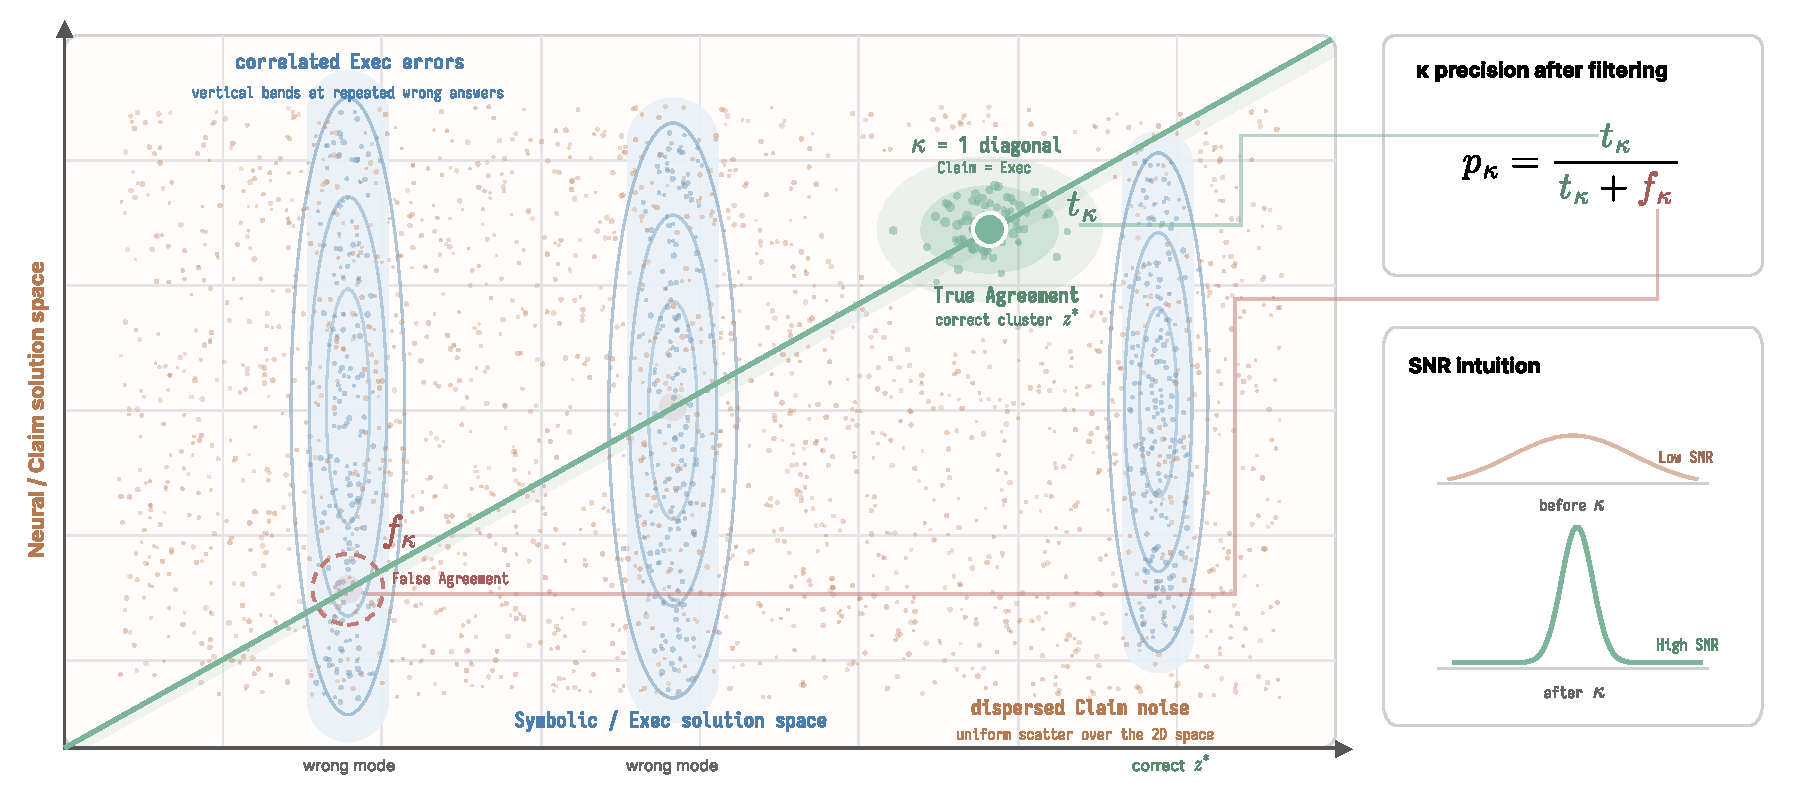
\includegraphics[width=\linewidth]{figures/precision.pdf}
    \caption{\textbf{Cross-channel precision filtering.} Left: $\kappa$ retains claim--execution agreement, which may be either true or false. Precision improves when correct executions are retained more often than incorrect ones, without an answer-dispersion assumption. Right: in the original aggregate, higher retained precision accompanies higher correlation and a \recheck{$4.1\times$} SNR-proxy improvement. Embedded statistics await the same aggregate recomputation as the red text.}
    \label{fig:precision-filtering}
\end{figure}

\subsection{\kgated{} Dual-Pathway \ccv{}}

Algorithm~\ref{alg:ccv} summarizes CCV. It uses claim-execution agreement as a precision gate, conceptually related to program-based consistency filtering~\citep{toh2024not}, but differs by combining agreement-gated consensus with output-pathway routing. The algorithm applies cross-channel agreement as a gate at two levels:

\begin{algorithm}[h]
\caption{$\kappa$-gated Dual-Pathway CCV}
\label{alg:ccv}
\begin{algorithmic}[1]
\REQUIRE Candidates $\{c_1, \ldots, c_K\}$, threshold $\tau_{\text{exec}}$
\FOR{each candidate $c_i$}
    \STATE $\kappa_i \gets \mathbf{1}[\text{claim}_i \approx \text{exec}_i \wedge \text{exec}_i \neq \bot]$
    \STATE $\text{score}_i \gets 0.5 \cdot |\text{claim\_cluster}_i| + \kappa_i \cdot (1 + |\text{exec\_cluster}_i|)$
\ENDFOR
\STATE $\mathcal{C}_\kappa \gets \{c_i : \kappa_i = 1\}$ \hfill $\triangleright$ self-consistent candidate pool
\IF{$\mathcal{C}_\kappa \neq \emptyset$}
    \STATE \textbf{return} $\text{claim}(\arg\max_{c_i \in \mathcal{C}_\kappa} \text{score}_i)$ \hfill $\triangleright$ \textit{Level 1: output neural claim}
\ELSE
    \STATE $z_{\text{exec}} \gets \text{mode}(\{\text{exec}_i : \text{exec}_i \neq \bot\})$
    \IF{$|\{i : \text{exec}_i = z_{\text{exec}}\}| \geq \tau_{\text{exec}}$}
        \STATE \textbf{return} $z_{\text{exec}}$ \hfill $\triangleright$ \textit{Level 2: fall back to symbolic execution}
    \ELSE
        \STATE \textbf{return} $\text{mode}(\{\text{claim}_i\})$ \hfill $\triangleright$ \textit{Level 3: fall back to claim majority}
    \ENDIF
\ENDIF
\end{algorithmic}
 \end{algorithm}

\paragraph{Candidate scoring (Lines 2--3).} The term $\kappa_i \cdot |\text{exec\_cluster}_i|$ realizes agreement-gated consensus: execution consensus is trusted only when accompanied by cross-layer agreement. The term $0.5 \cdot |\text{claim\_cluster}|$ provides a baseline surface signal. Raw execution cluster size receives zero weight---our learned ablation in Section~\ref{sec:learned} confirms this design choice.

\paragraph{Output pathway routing (Lines 6--12).} When self-consistent candidates exist ($\mathcal{C}_\kappa$ is non-empty), the algorithm outputs the neural claim. When cross-layer agreement collapses globally, it falls back to symbolic execution consensus, but only if the execution cluster is sufficiently large ($\geq \tau_{\text{exec}}$). An empty agreement pool does not identify which channel is wrong; the execution threshold is a heuristic fallback, and the regressions in Section~\ref{sec:errors} show its limits.

\textbf{Complexity and scope.} Aggregation takes $O(K)$ time after answer normalization and clustering. On an existing \sketch{} candidate pool, verification requires no additional model calls; the generator still requires LoRA SFT and teacher-assisted reformatting, so \ccv{} is not a drop-in verifier for arbitrary unstructured pools. Aggregation costs 2--4 ms per question on one CPU core (\recheck{4--7 s} for the original pool); external DSL execution is shared with execution-based baselines. Appendix~\ref{app:costs} separates these costs from generator training and external scoring. We select $\tau_{\text{exec}}$ on development data and examine the other fixed matching and scoring constants in Appendix~\ref{app:constants}.

% ===========================================================================
\section{Experiments}
\label{sec:experiments}
% ===========================================================================

\subsection{Setup}

\paragraph{Models and training.} Our primary generator is Qwen3.5-9B, fine-tuned with LoRA ($r{=}8, \alpha{=}16$) on 2,012 executor-validated Geometry3K training examples. The training data was constructed by reformatting Qwen3-VL CoT traces into the \sketch{} format using DeepSeek V4 Pro. We also evaluate Gemma4-E4B to test cross-model generalization. Training was conducted using LLaMA-Factory with bf16 on 8 NVIDIA 4090 GPUs.

\begin{table}[h]
\centering
\caption{Test benchmark suite: three primary benchmarks and a reference superset. MathVista GPS denotes its geometry problem solving subset; GPS-clean is a strict subset of GPS-full. OOD denotes out-of-distribution evaluation.}
\label{tab:benchmarks}
\small
\begin{tabular}{lccc}
\toprule
Benchmark & Lang. & $N$ & Role \\
\midrule
Geometry3K test~\citep{lu2021inter} & EN & 601 & In-distribution \\
GeoQA test~\citep{chen2021geoqa} & ZH & 754 & Cross-lingual OOD \\
MathVista-GPS clean (GPS-c)~\citep{lu2023mathvista} & EN & 146 & Cross-domain OOD \\
MathVista-GPS (GPS-full)~\citep{lu2023mathvista} & EN & 208 & \shortstack{Reference\\(superset of GPS-clean)} \\
\bottomrule
\end{tabular}
\par\smallskip
\begin{minipage}{\linewidth}\footnotesize
GPS-clean contains 146 of the 208 GPS-full questions. GPS-full is reported separately and is excluded from the main aggregate to avoid duplicate counting.
\end{minipage}
\end{table}

\paragraph{Evaluation protocol.} Table~\ref{tab:benchmarks} summarizes three primary benchmarks: Geometry3K test, GeoQA test, and GPS-clean, with GPS-full reported for reference. ``All'' aggregates only the three primary sets; heldout/OOD uses Geometry3K qid$\geq300$, GeoQA test, and GPS-clean, excluding both the Geometry3K dev split (qid$<300$) and GPS-full. Red values preserve original overlapping-pool statistics and await recomputation; they are not recomputed estimates for the revised aggregate. We use a frozen-rollout protocol with $K{=}16$ candidates, temperature $0.8$, and top-$p$ $0.95$. All verification methods operate on the same rollout pool, denoted s240 for the frozen Qwen rollout pool. The execution fallback threshold $\tau_{\text{exec}}{=}9$ was selected on a 300-question development split of Geometry3K and held fixed across all benchmarks and models.

\subsection{Main Results}

\begin{figure*}[t]
    \centering
    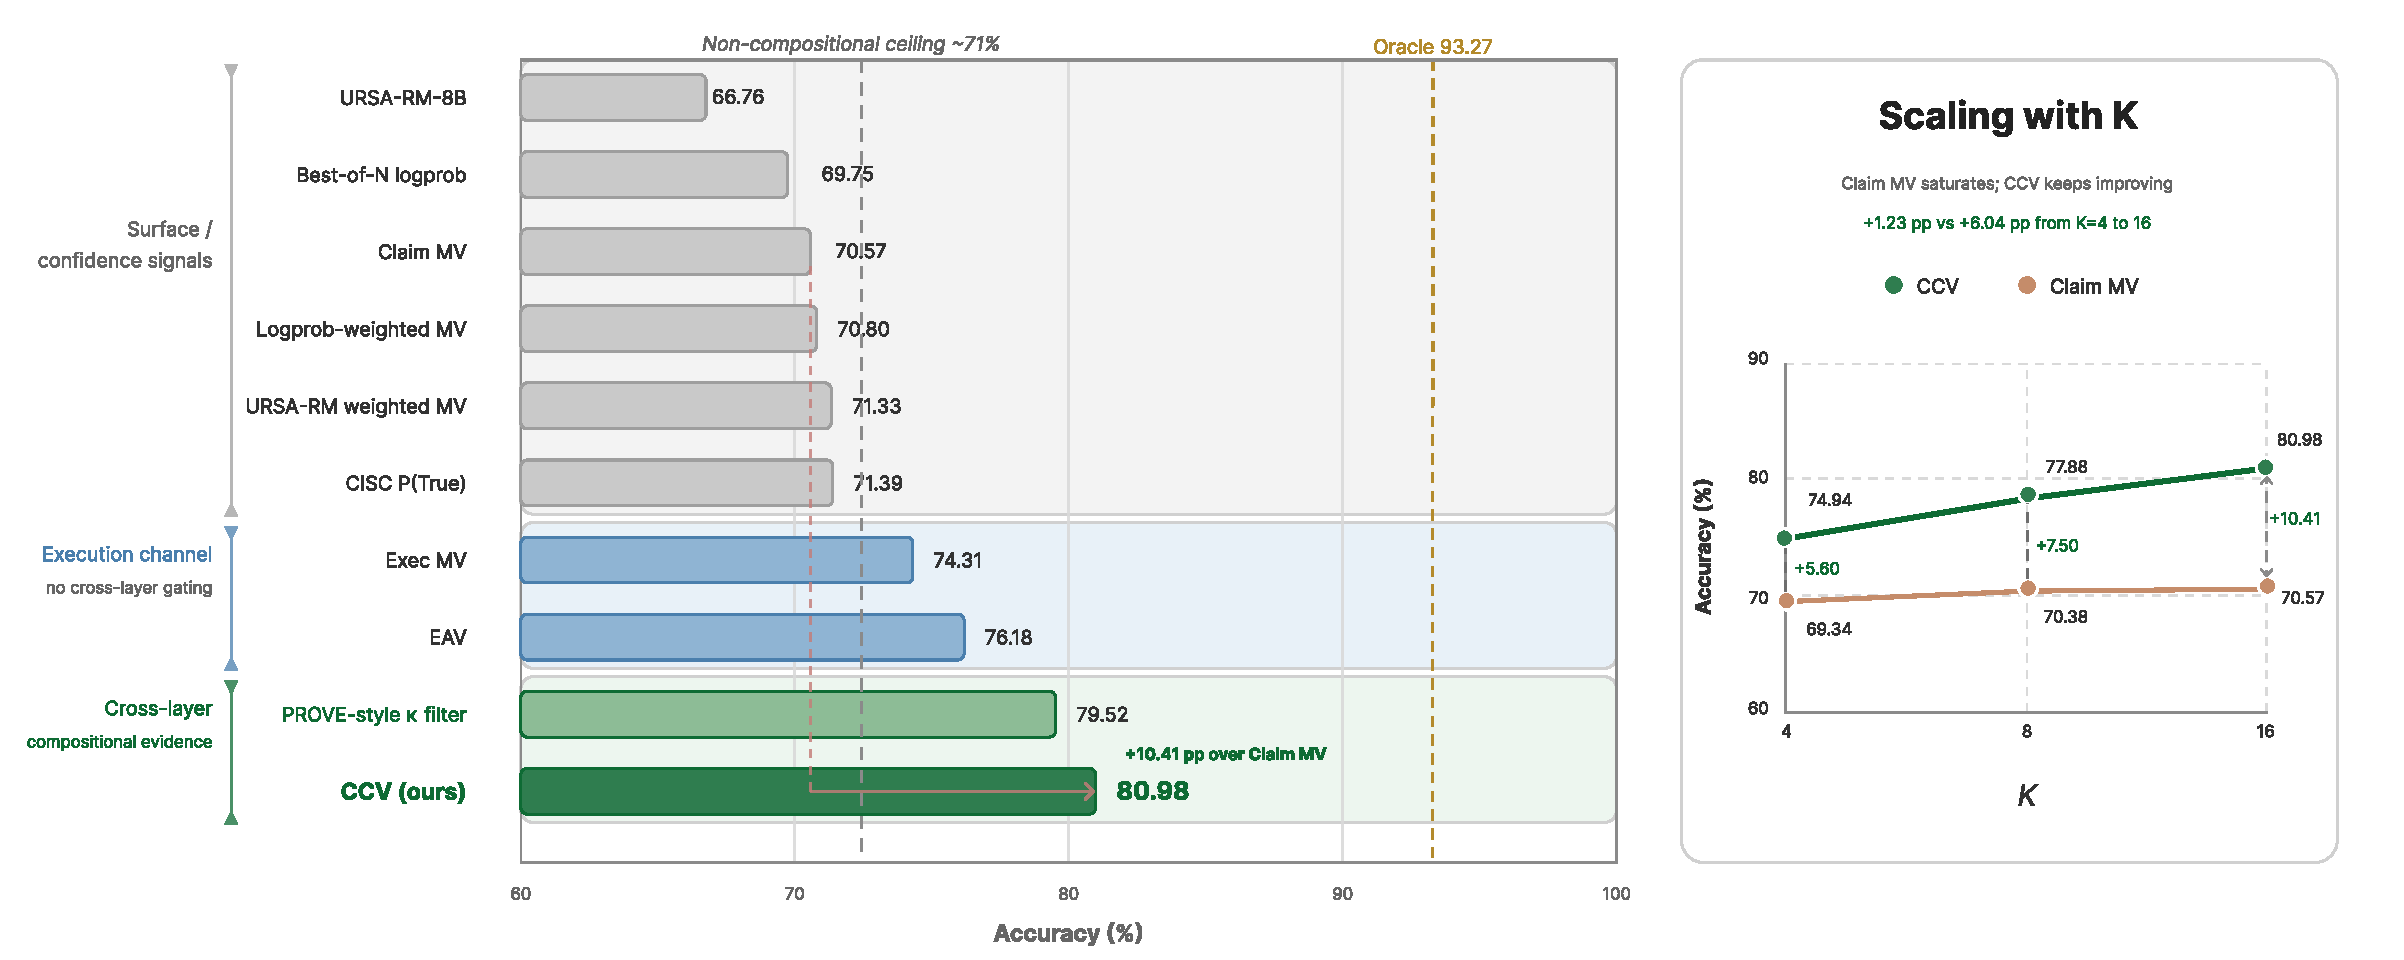
\includegraphics[width=0.72\textwidth]{figures/figure3.pdf}
    \caption{\textbf{Evidence ladder and $K$ scaling.} Surface and confidence-based selectors cluster near \recheck{70--71\%}, execution-only methods improve moderately, and cross-layer compositional verification produces the main jump to \recheck{79--81\%}. As $K$ increases, the \ccv{} gain over Claim MV grows, indicating that compositional verification unlocks additional rollout diversity. Embedded aggregate statistics await recomputation without GPS-full.}
    \label{fig:evidence-scaling}
\end{figure*}

Execution-Answer Voting (EAV) is the execution-first priority baseline. Figure~\ref{fig:evidence-scaling} visualizes the same evidence ladder and $K$-scaling trend, while Table~\ref{tab:main} reports the full benchmark breakdown. The four surface and confidence-based selectors---Claim MV, logprob-weighted MV, CISC, and URSA-RM weighted MV---all lie in a narrow \recheck{70.57--71.39}\% band, despite spanning self-confidence weighting and an external learned PRM. The learned ablation in Section~\ref{sec:learned} shows a similar range for logprob-based best-of-$N$ and learned surface+execution feature selectors. Even URSA-RM, the strongest external scorer, achieves only $+\recheck{0.76}\pp$ over Claim MV when used for weighted voting. Execution-only methods improve to \recheck{74--76\%}, but the large jump appears only when cross-layer agreement is used as a compositional signal: a PROVE-style $\kappa$ filter reaches \recheck{79.52}\%, and \ccv{} reaches \recheck{80.98}\%, a $+\recheck{10.41}\pp$ improvement over Claim MV and $+\recheck{4.80}\pp$ over EAV.

The original paired per-question analysis over \recheck{1,709} entries reported the following gains, confidence intervals, and tests, all of which require recomputation without GPS-full: \ccv{} improves over Claim MV by $+\recheck{10.42}\pp$ (95\% paired bootstrap CI $[\recheck{8.48},\recheck{12.40}]\pp$; exact McNemar $p<\recheck{10^{-12}}$) and over EAV by $+\recheck{4.80}\pp$ (95\% CI $[\recheck{3.39},\recheck{6.26}]\pp$; exact McNemar $p=\recheck{5.7{\times}10^{-11}}$). The original heldout analysis also reports gains away from the development split: on the disjoint heldout/OOD split (excluding dev 300), \ccv{} reaches \recheck{81.93}\%. Finally, a sweep over the development-selected threshold, $\tau_{\text{exec}}$, reports a broad plateau: across $\tau_{\text{exec}}=5\ldots14$, dev accuracy varies by 1.00$\pp$ and heldout/OOD accuracy by \recheck{1.06}$\pp$ (Appendix~\ref{app:tau-sensitivity}). The $\kappa$ matching threshold itself is also stable: varying the candidate-level relative tolerance around the default leaves \ccv{} accuracy unchanged on the full s240 pool (Appendix~\ref{app:kappa-threshold}).

\afterpage{%
\begin{table*}[t]
\centering
\caption{Evidence ladder across verification signal types ($K{=}16$). All aggregates G3K, GeoQA, and GPS-c only; GPS (GPS-full), separated on the right, is a reference superset excluded from All. Red All values await recomputation. Bold marks the best non-oracle method in each column; PROVE-style filtering leads on GeoQA. Surface/confidence methods, including learned PRM scores and self-judged confidence, cluster near \recheck{70--71\%}. Execution-only signals improve moderately. Cross-layer compositional verification produces the large jump to \recheck{79--81\%}.}
\label{tab:main}
\small
\begin{tabular}{llcccc|c}
\toprule
Method & Type & G3K & GeoQA & GPS-c & All & GPS \\
\midrule
\multicolumn{7}{l}{\textit{Surface / confidence signals}} \\
Claim MV & consensus & 66.72 & 73.61 & 72.60 & \recheck{70.57} & 69.23 \\
Logprob-weighted MV & weighted consensus & 66.56 & 73.87 & 72.60 & \recheck{70.80} & 70.67 \\
CISC $P(\mathrm{True})$-weighted & confidence consensus & 68.05 & 74.27 & 72.60 & \recheck{71.39} & 69.71 \\
URSA-RM weighted MV & learned verifier & 62.73 & 75.60 & 79.45 & \recheck{71.33} & 75.00 \\
\midrule
\multicolumn{7}{l}{\textit{Execution channel without cross-layer gating}} \\
Exec MV & exec consensus & 72.71 & 75.60 & 76.71 & \recheck{74.31} & 72.60 \\
EAV & exec-first priority & 74.04 & 77.72 & 77.40 & \recheck{76.18} & 75.96 \\
\midrule
\multicolumn{7}{l}{\textit{Cross-layer compositional signals}} \\
PROVE-style $\kappa$ filter & binary agreement & 76.54 & \textbf{82.10} & 81.51 & \recheck{79.52} & 77.40 \\
\ccv{} (ours) & gated + routing & \textbf{78.54} & 81.83 & \textbf{86.30} & \recheck{\textbf{80.98}} & \textbf{81.25} \\
\midrule
Oracle & upper bound & 93.51 & 93.50 & 91.78 & \recheck{93.27} & 92.79 \\
\bottomrule
\end{tabular}
\end{table*}
}

\subsection{Cross-Model Generalization}
\label{sec:cross-model-generalization}

To test whether \ccv{}'s gains depend on the specific base model, we repeat the full evaluation protocol with Gemma4-E4B, a 4B-parameter multimodal model with substantially weaker geometry reasoning capacity. The Gemma4 model achieves comparable \sketch{} format compliance to the Qwen model, so this experiment is a confirmation of the verification mechanism rather than a new generator contribution.

Table~\ref{tab:cross-model} reports the cross-model evidence ladder using the same $\tau_{\text{exec}}{=}9$ for both models. First, the absolute accuracy gap is large: Claim MV drops from \recheck{70.57}\% on Qwen3.5-9B to \recheck{44.94}\% on Gemma4-E4B, consistent with the capacity difference. Second, the \ccv{} gain pattern is preserved: \ccv{} improves over Claim MV by $+\recheck{10.41}\pp$ on Qwen and $+\recheck{7.84}\pp$ on Gemma4. The Gemma4 result is especially diagnostic because its execution pathway alone is worse than the claim pathway (Exec MV \recheck{41.08}\% vs Claim MV \recheck{44.94}\%), making EAV ineffective (\recheck{44.88}\%). Yet \ccv{} still reaches \recheck{52.78}\%, showing that it exploits structural cross-channel agreement rather than the raw accuracy advantage of execution votes.

The precision-filtering pattern also replicates quantitatively: $\kappa$-filtering yields nearly identical precision gains across models ($+\recheck{25.40}\pp$ vs $+\recheck{26.38}\pp$), and the counterintuitive correlation pattern repeats ($\rho_\kappa>\rho_e$ while SNR improves; Table~\ref{tab:cross-model-diagnostics}). This supports transfer between the two tested model families; it does not establish model-independent gains. The \ccv{} advantage also scales with $K$ on both Qwen and Gemma4 (Appendix~\ref{app:diagnostics}, Appendix~\ref{app:gemma-k-scaling}).

\subsection{$K$ Scaling Analysis}

Figure~\ref{fig:evidence-scaling} shows that the \ccv{} advantage scales with $K$: the gain over Claim MV grows from $+$\recheck{5.60}$\pp$ at $K{=}4$ to $+$\recheck{10.41}$\pp$ at $K{=}16$ (tabulated in Appendix~\ref{app:diagnostics}). Surface consensus saturates quickly (Claim MV gains only $+$\recheck{1.23}$\pp$ from $K{=}4$ to 16), while compositional verification continues extracting signal from larger candidate pools.

As a negative control, VGF consensus---another within-layer signal---not only fails to help but \emph{hurts} performance when added (from \recheck{80.05}\% to \recheck{79.93}\%). This reinforces the central finding: within-layer consensus---whether the layer is claim, execution, or VGF---is vulnerable to correlated perception errors. In these comparisons, the substantial gains come from cross-layer gating.

\subsection{Learned Feature Ablation}
\label{sec:learned}

To validate that the compositional features carry the transferable verification signal---not just that our specific CCV rule is effective---we train candidate-level logistic regression classifiers on Geometry3K dev (300 questions) and evaluate on disjoint OOD benchmarks.

Table~\ref{tab:learned} reports the full ablation. In this ablation, the substantial heldout gains come from compositional features: logprob best-of-$N$, surface features, and surface+execution features remain near Claim MV (\recheck{71.11--71.86}\% OOD), while adding cross-layer features jumps to \recheck{79.85}\% OOD and C-only features reach \recheck{81.02}\%. The learned model rediscovers the gating principle: raw $\text{exec\_cluster\_size}$ has a negative coefficient ($-2.40$), while $\kappa \times \text{exec\_cluster}$ is strongly positive ($+1.96$). A simple rule is therefore enough: PROVE-style $\kappa$ filtering reaches \recheck{81.02}\% OOD, and dual-output \ccv{} reaches \recheck{81.93}\% OOD.

\subsection{Recoveries and Regressions}
\label{sec:errors}

\ccv{} changes answers in both directions. Relative to Claim MV, it records \recheck{237} wins and \recheck{59} losses (\recheck{4.02:1}); relative to EAV, it records \recheck{121} wins and \recheck{39} losses (\recheck{3.10:1}). The per-benchmark net gains over Claim MV are positive, ranging from $+8.22\pp$ on GeoQA to $+13.70\pp$ on GPS-clean. Appendix~\ref{app:regressions} reports both $2\times2$ exchange tables and the regression categories.

The recovery-only taxonomy considers \recheck{355} EAV failures with an oracle-correct candidate. Wrong execution consensus accounts for \recheck{305/355} (\recheck{86\%}). For the Exec\ding{55}\,Claim\ding{51} subtype, where the execution majority is wrong but the claim majority is correct, \ccv{} recovers \recheck{123/139} (\recheck{88.5\%}). The Exec\ding{55}\,Claim\ding{55} subtype remains difficult (\recheck{8.3\%} recovered). These subtype counts and the paired exchange tables come from different reported analyses and must be reconciled in the aggregate audit; the flow figure describes recoveries, not net gains. Among self-consistent candidates, reliability rises from \recheck{19\%} at execution cluster size 1 to \recheck{93\%} at size 8+, supporting the combination of agreement and consensus.

Regressions expose three limits. False $\kappa$ agreement explains \recheck{26/59} losses against Claim MV and \recheck{30/39} against EAV, often with small wrong agreement groups (median sizes \recheck{3} and \recheck{2}, respectively). Incorrect fallback execution consensus explains \recheck{33} losses against Claim MV: none of their candidates executes to the correct answer, and \recheck{15} have unanimous 16/16 execution consensus. Threshold effects account for \recheck{7} losses against EAV. Agreement and strong fallback consensus can both preserve shared errors.

% ===========================================================================
\section{Related Work}
\label{sec:related}
% ===========================================================================

Geometry reasoning systems mainly improve the generator side of the problem. Specialized VLMs such as G-LLaVA~\citep{gao2023g}, GeoX~\citep{xia2024geox}, and MAVIS~\citep{zhang2024mavis} strengthen multimodal geometry solving on benchmarks such as Geometry3K~\citep{lu2021inter} and GeoQA~\citep{chen2021geoqa}. Neuro-symbolic solvers such as AlphaGeometry~\citep{trinh2024solving,chervonyi2025gold} and FormalGeo~\citep{zhang2023formalgeo} use symbolic structure to derive proofs or answers. Our work is complementary: it assumes a candidate pool already exists and studies how to verify candidates when shared diagram perception makes their errors correlated.

Test-time verification is usually based on either consensus or learned scoring. Self-consistency~\citep{wang2022self}, universal self-consistency~\citep{chen2023universal}, and confidence-weighted CISC~\citep{taubenfeld2025confidence} aggregate opaque answer votes, which works best when sampled errors are sufficiently independent. Learned verifiers, including ORMs/PRMs~\citep{cobbe2021training,uesato2022solving,lightman2023let,wang2024math}, GenRM~\citep{zhang2024generative}, URSA-RM~\citep{luo2025ursa}, and VisualPRM~\citep{wang2025visualprm}, train external scorers and add verifier-specific data or inference. \ccv{} differs from both paradigms by deriving verification signal from structure already present inside each candidate.

The closest line of work uses programs or error-correlation analysis to diagnose voting failures. PROVE~\citep{toh2024not} filters candidates whose translated Python output matches the natural-language answer, a binary consistency signal analogous to $\kappa$. Our framework generalizes this idea to geometry-specific neuro-symbolic outputs, where VGF, typed DSL, deterministic execution, and neural claims form a hierarchy of cross-layer signals. \citet{nitarach2026model} show that correlated errors limit majority voting; \ccv{} targets this regime directly by gating consensus through cross-channel agreement rather than trying to decorrelate samples.

% ===========================================================================
\section{Limitations}
\label{sec:limitations}

\paragraph{Coupled generation.}
The claim and DSL are produced by one autoregressive model, and the claim conditions on the DSL source. Their mean within-question correctness correlation is $\phi=\recheck{0.325}$; they are not independent solutions. The likelihood-ratio condition characterizes retained-candidate precision, while pool-level selection gains remain empirical and can fail under correlated false agreement.

\paragraph{Generator and teacher dependence.}
The training-free verifier operates only once a \sketch{} pool exists. Our generators require LoRA SFT on teacher-assisted reformatted traces; this preparation is part of the method's cost and limits applicability to arbitrary existing candidate pools. Closed-source models might emit \sketch{} through few-shot prompting, but we have not tested this and make no performance claim for them.

\paragraph{Format degradation and fallback.}
Malformed or non-executable programs cannot contribute execution votes and are excluded from $\kappa$ agreement. Format degradation therefore shrinks the agreement pool and can trigger fallback, rather than silently treating a failed execution as concordant. This handling does not make fallback reliable: well-formed programs can execute incorrect premises, and strong execution consensus can still be wrong.

\paragraph{Task and domain boundaries.}
We validate numeric and multiple-choice geometry reasoning on two open-weight model families. Transfer to chart/table question answering, physics diagrams, or code generation is a hypothesis that should first be tested by estimating the agreement likelihood ratio on labeled pools. A ratio near one predicts little precision benefit. Open-ended geometry proofs require agreement at the level of proof-checker judgments, replacing numeric equality; that is a method extension, not a change of tolerance.

\paragraph{Selection-only headroom.}
Only \recheck{8.3\%} of the reported Exec\ding{55}\,Claim\ding{55} subtype is recovered. Selection cannot produce an answer absent from the candidate pool: reported oracle accuracies are \recheck{93.27\%} for Qwen and \recheck{91.75\%} for Gemma. This separates remaining error into cases where no correct candidate is available and cases where a correct candidate exists but the selector misses it. Premise verification or improved generation is needed to address the first component; the exchange tables characterize risks in the second.

\section{Conclusion}

\sketch{} exposes a claim and an externally executed program result for each geometry candidate. \ccv{} is a training-free verifier over these structured pools, with no additional model calls at verification time. Its precision benefit requires agreement to be more likely for correct executions than for incorrect ones, a condition compatible with positively correlated channels and substantial false agreement. The reported geometry comparisons place non-compositional methods around \recheck{70--71\%} and cross-channel methods around \recheck{79--81\%}, with both recoveries and regressions; aggregate values await recomputation on three benchmarks, with GPS-full reported for reference. Benefits beyond geometry remain a hypothesis. A falsifiable next step is to measure the likelihood ratio on labeled chart/table QA, physics-diagram, and code-generation pools before testing pool-level selection gains.

\paragraph{Planned release.}
We will release evaluation and aggregation scripts, frozen candidate pools and per-question selections, external scorer files, and audit scripts to support reproducibility of the verification comparisons.

% ===========================================================================
% References - placeholder entries
% ===========================================================================

\bibliographystyle{plainnat}
\bibliography{references}

%%%%%%%%%%%%%%%%%%%%%%%%%%%%%%%%%%%%%%%%%%%%%%%%%%%%%%%%%%%%
\appendix
\numberwithin{equation}{section}
\numberwithin{table}{section}
\numberwithin{figure}{section}

\section{Training Data Construction}
\label{app:data-construction}

Table~\ref{tab:data-construction} summarizes the full construction pipeline for the 2,012-example SFT set. We start from the official Geometry3K~\citep{lu2021inter} training split, use the geometry3k subset of Nemotron-Image-Training-v3~\citep{blakeman2025nvidia} as the Qwen3-VL-235B-A22B-Thinking CoT source, reformat each matched trace into the \sketch{} VGF+DSL+answer format with DeepSeek V4 Pro, and retain only examples whose DSL executes and matches the official answer. The reformatting stage is text-only: the expensive visual reasoning is supplied by the Qwen3-VL CoT trace, while the official gold answer is used as the final target for machine-checkable reformatting.

\begin{table}[h]
\centering
\caption{Training data construction and filtering. Percentages are relative to the 2,078 matched CoT rows unless otherwise noted.}
\label{tab:data-construction}
\small
\begin{tabular}{lrr}
\toprule
Stage & Count & Rate \\
\midrule
Official Geometry3K train rows & 2,101 & -- \\
Matched Qwen3-VL CoT traces & 2,078 & 98.91\% of official \\
Qwen3-VL boxed-answer correct & 2,065 & 99.37\% \\
DeepSeek V4 Pro reformat attempts & 2,078 & 100.00\% \\
Strict validator pass & 1,963 & 94.47\% \\
Recovered by tolerant VGF normalization & 49 & 2.36\% \\
Final executor-validated SFT rows & 2,012 & 96.82\% \\
\midrule
Filtered: execution-answer mismatch & 61 & 2.94\% \\
Filtered: DSL execution/safety error & 5 & 0.24\% \\
\bottomrule
\end{tabular}
\end{table}

The final 66 filtered examples consist of 61 execution-answer mismatches and five DSL execution/safety failures: one undefined \texttt{UB}, one undefined \texttt{z}, one undefined \texttt{m}, and two blocked-token errors. The tolerant VGF pass clears unsupported or over-arity visual facts only when the DSL and answer remain executor-valid; a final post-processing pass keeps 2,012 rows, with 41 DSL snippets changed by the sanitizer and 6 VGF lists cleared.

\section{Data Construction Prompts}
\label{app:prompts}

\paragraph{Stage 1: stored source prompt for frontier CoT traces.}
We did not rerun Qwen3-VL-235B-A22B-Thinking for this paper. We use an existing CoT source whose stored user messages follow the problem image plus the following prompt pattern:
\begin{verbatim}
Solve this geometry problem. Study the diagram and select
the correct answer.

{problem_text}
{choices}

Do not explain your answer but write only the answer label
(A, B, ...) in this format:
Answer: \boxed{...}.
\end{verbatim}

\paragraph{Stage 2: VGF+DSL reformatting.}
DeepSeek V4 Pro receives no image input. It reformats the official problem, choices, official answer, and Qwen3-VL CoT into the target \sketch{} format using the following template:
\begin{verbatim}
Convert the provided Qwen3-VL-235B natural-language geometry
chain-of-thought into the target VGF+DSL format.
Do not solve from scratch. Use the teacher CoT as the visual
and reasoning evidence, and use the official gold answer as
the final target.
Return exactly three sections in this order and no extra sections:
[VGF]
[DSL]
[Final Answer]

[VGF] rules:
Output a raw JSON list only. Do not use markdown fences.
Each item must be {"relation": <relation>,
"entities": [<tokens>]} with exact relation arity.
Allowed relations: {allowed_vgf_relations}.
Relation arities: {relation_arities}.
For unary shape relations, put the whole object in one entity
token, e.g.
{"relation":"parallelogram","entities":["MNPQ"]}.
Use at most 4 facts to stay safely under the validator limit
of 5 facts.
Use [] if no reliable visual fact is needed.

[DSL] rules:
Output executable Python assignment statements only.
Do not use markdown fences.
Do not include comments or prose.
Never write import statements, including 'from math import ...'.
Math functions are already available by name.
Every variable must be assigned before it is used.
Do not write placeholder equations with unknown symbols.
The final assignment must define a variable named answer.
The value of answer must evaluate to the official gold option
value; use the teacher CoT equations to derive that value.
Allowed math names: sqrt, pi, sin, cos, tan, radians, degrees,
asin, acos, atan, abs, min, max, round.
Do not read files, import modules, call external tools, or use
input/output functions.
[Final Answer] must be exactly the official gold option letter:
{gold}.
In [DSL], set answer to the numeric or symbolic value of
option {gold}:
{gold_value}.

Official problem:
{problem_text}
{choices}

Official gold answer: {gold}
Official gold option value: {gold_value}
Teacher boxed answer: {qwen_boxed_answer}

Teacher NL CoT:
{qwen_cot}
\end{verbatim}

\section{$\tau_{\text{exec}}$ Sensitivity}
\label{app:tau-sensitivity}

The development-selected parameter in \ccv{} is the execution-majority threshold $\tau_{\text{exec}}$, used only when the $\kappa$-pool is empty. We sweep $\tau_{\text{exec}}=1\ldots16$ on the main Qwen3.5-9B s240 $K{=}16$ rollout pool, using the same split protocol as the main paper: Geometry3K qid$<300$ for dev, and Geometry3K qid$\geq300$ plus GeoQA and GPS-clean for heldout/OOD evaluation; GPS-full is excluded. Figure~\ref{fig:tau-sensitivity} plots the full sweep, and Table~\ref{tab:tau-sensitivity} reports selected points. We use the resulting $\tau_{\text{exec}}{=}9$ for both Qwen3.5-9B and Gemma4-E4B.

\begin{figure}[h]
    \centering
    \definecolor{tauDev}{HTML}{1F77B4}
\definecolor{tauOod}{HTML}{D62728}
\definecolor{tauBand}{HTML}{EFEFEF}

\begin{tikzpicture}[
  x=0.52cm,
  y=0.58cm,
  font=\sffamily,
  axis/.style={draw=black!50, line width=0.55pt},
  grid/.style={draw=black!14, line width=0.35pt},
  ticklabel/.style={font=\sffamily\scriptsize, text=black!62},
  legend/.style={font=\sffamily\scriptsize, text=black!75, anchor=west}
]

\fill[tauBand] (5,0.40) rectangle (14,7.35);
\node[ticklabel, anchor=south] at (9.5,7.35) {$\tau_{\mathrm{exec}}=5\ldots14$};

\foreach \y/\lab in {1/76,3/78,5/80,7/82} {
  \draw[grid] (1,\y) -- (16,\y);
  \node[ticklabel, anchor=east] at (0.70,\y) {\lab};
}
\draw[axis] (1,0.40) -- (16,0.40);
\draw[axis] (1,0.40) -- (1,7.35);

\foreach \x in {1,...,16} {
  \draw[axis] (\x,0.40) -- (\x,0.28);
  \node[ticklabel, anchor=north] at (\x,0.20) {\x};
}

\draw[tauDev, line width=1.2pt] plot coordinates {(1,1.67) (2,1.67) (3,1.67) (4,1.67) (5,2.00) (6,2.00) (7,2.00) (8,2.00) (9,2.00) (10,2.00) (11,2.00) (12,1.67) (13,1.33) (14,1.00) (15,0.67) (16,0.67)};
\draw[tauOod, line width=1.2pt] plot coordinates {(1,5.13) (2,5.20) (3,5.20) (4,5.41) (5,5.77) (6,5.91) (7,6.05) (8,6.19) (9,6.83) (10,6.83) (11,6.76) (12,6.41) (13,6.26) (14,6.33) (15,6.12) (16,6.19)};

\foreach \x/\y in {1/1.67,2/1.67,3/1.67,4/1.67,5/2.00,6/2.00,7/2.00,8/2.00,9/2.00,10/2.00,11/2.00,12/1.67,13/1.33,14/1.00,15/0.67,16/0.67} {
  \fill[tauDev] (\x,\y) circle (2.0pt);
}
\foreach \x/\y in {1/5.13,2/5.20,3/5.20,4/5.41,5/5.77,6/5.91,7/6.05,8/6.19,9/6.83,10/6.83,11/6.76,12/6.41,13/6.26,14/6.33,15/6.12,16/6.19} {
  \fill[tauOod] (\x,\y) rectangle ++(0.13,0.13);
}

\node[ticklabel, anchor=north] at (8.5,-0.48) {$\tau_{\mathrm{exec}}$};
\node[ticklabel, rotate=90, anchor=south] at (-0.35,3.95) {CCV accuracy (\%)};
\draw[tauDev, line width=1.2pt] (11.6,1.28) -- (12.4,1.28);
\fill[tauDev] (12.0,1.28) circle (2.0pt);
\node[legend] at (12.55,1.28) {Geometry3K dev300};
\draw[tauOod, line width=1.2pt] (11.6,0.78) -- (12.4,0.78);
\fill[tauOod] (11.94,0.72) rectangle ++(0.13,0.13);
\node[legend] at (12.55,0.78) {Heldout+OOD};

\end{tikzpicture}

    \caption{\textbf{Sensitivity to $\tau_{\text{exec}}$.} \ccv{} is stable over a broad range of execution thresholds. In the plateau $\tau_{\text{exec}}=5\ldots14$, dev accuracy varies from 76.00\% to 77.00\%, and heldout/OOD accuracy varies from \recheck{80.77\%} to \recheck{81.83\%}. Embedded curve statistics await recomputation without GPS-full.}
    \label{fig:tau-sensitivity}
\end{figure}

\begin{table}[h]
\centering
\caption{Selected points from the $\tau_{\text{exec}}$ sweep (full curve in the figure above). The dev-selected threshold is $\tau_{\text{exec}}=9$.}
\label{tab:tau-sensitivity}
\small
\begin{tabular}{rccc}
\toprule
$\tau_{\text{exec}}$ & Dev@300 & Heldout/OOD & All \\
\midrule
1 (no threshold) & 76.67 & \recheck{80.13} & \recheck{79.52} \\
9 (selected) & \textbf{77.00} & \recheck{\textbf{81.83}} & \recheck{\textbf{80.98}} \\
16 (maximum) & 75.67 & \recheck{81.19} & \recheck{80.22} \\
\bottomrule
\end{tabular}
\end{table}

\section{Additional Diagnostics}
\label{app:diagnostics}

This appendix contains the diagnostic tables and flow visualization referenced by the main experimental analysis. Table~\ref{tab:cross-model-diagnostics} reports the precision-filtering statistics behind the cross-model claim, Table~\ref{tab:scaling} gives the exact Qwen $K$-scaling values summarized in Figure~\ref{fig:evidence-scaling}, Table~\ref{tab:learned} gives the learned feature ablation, and Figure~\ref{fig:routing-sankey} visualizes the error taxonomy and routing behavior.

\begin{table}[h]
\centering
\caption{Cross-model diagnostic for the precision-filtering mechanism. The $\kappa$-filtered pool is more correlated than the raw execution pool, but its much higher per-candidate precision improves the effective verification signal.}
\label{tab:cross-model-diagnostics}
\small
\resizebox{\linewidth}{!}{
\begin{tabular}{lccccccc}
\toprule
Model & $p_e$ (\%) & $p_\kappa$ (\%) & $\Delta p$ (pp) & $\rho_e$ & $\rho_\kappa$ & mean $K_\kappa$ & SNR raw$\rightarrow\kappa$ \\
\midrule
Qwen3.5-9B & \recheck{61.70} & \recheck{87.10} & \recheck{$+25.40$} & \recheck{0.526} & \recheck{0.646} & \recheck{9.09} & \recheck{0.32$\rightarrow$1.33} \\
Gemma4-E4B & \recheck{33.43} & \recheck{59.81} & \recheck{$+26.38$} & \recheck{0.504} & \recheck{0.630} & \recheck{5.77} & \recheck{$-$0.48$\rightarrow$0.24} \\
\bottomrule
\end{tabular}
}
\end{table}

\begin{table}[h]
\centering
\caption{Performance across $K$ for the three primary benchmarks, with GPS-full reported separately for reference. The original aggregate values shown here await recomputation excluding GPS-full.}
\label{tab:scaling}
\small
\begin{tabular}{rccccc}
\toprule
$K$ & Claim MV & Exec MV & \ccv{} & Oracle & \ccv{} $-$ Claim MV \\
\midrule
4 & \recheck{69.34} & \recheck{68.98} & \recheck{74.94} & \recheck{84.74} & \recheck{$+$5.60} \\
8 & \recheck{70.38} & \recheck{72.43} & \recheck{77.88} & \recheck{89.89} & \recheck{$+$7.50} \\
16 & \recheck{70.57} & \recheck{74.31} & \recheck{80.98} & \recheck{93.27} & \recheck{$+$10.41} \\
\bottomrule
\end{tabular}
\end{table}

\begin{table}[h]
\centering
\caption{Compositional feature ablation. ``S'' = standard features (logprob, claim cluster), ``E'' = execution features, ``C'' = compositional cross-layer features ($\kappa$, $\kappa \times \text{exec\_cluster}$, $\mu$, $\kappa \times \mu$, sc\_rate). The last column reports OOD gain over Claim MV.}
\label{tab:learned}
\small
\begin{tabular}{lcccc}
\toprule
Method / Features & Dev@300 & OOD & All & \shortstack{$\Delta$ OOD\\vs Claim MV} \\
\midrule
Claim MV (reference) & 66.67 & \recheck{71.77} & \recheck{70.57} & \recheck{0.00} \\
Best-of-$N$ (logprob) & 66.00 & \recheck{71.11} & \recheck{69.75} & \recheck{$-$0.67} \\
LogReg S-only & 67.00 & \recheck{71.86} & \recheck{70.74} & \recheck{$+$0.08} \\
LogReg S+E & 66.33 & \recheck{71.69} & \recheck{70.63} & \recheck{$-$0.08} \\
LogReg S+E+C & 74.67 & \recheck{79.85} & \recheck{78.47} & \recheck{$+$8.08} \\
LogReg C-only & 75.33 & \recheck{81.02} & \recheck{79.64} & \recheck{$+$9.24} \\
\midrule
PROVE-style $\kappa$ filter (rule) & 75.00 & \recheck{81.02} & \recheck{79.52} & \recheck{$+$9.24} \\
Dual-output \ccv{} (ours, rule) & 77.00 & \recheck{81.93} & \recheck{80.98} & \recheck{$+$10.16} \\
\bottomrule
\end{tabular}
\end{table}

\begin{figure*}[t]
    \centering
    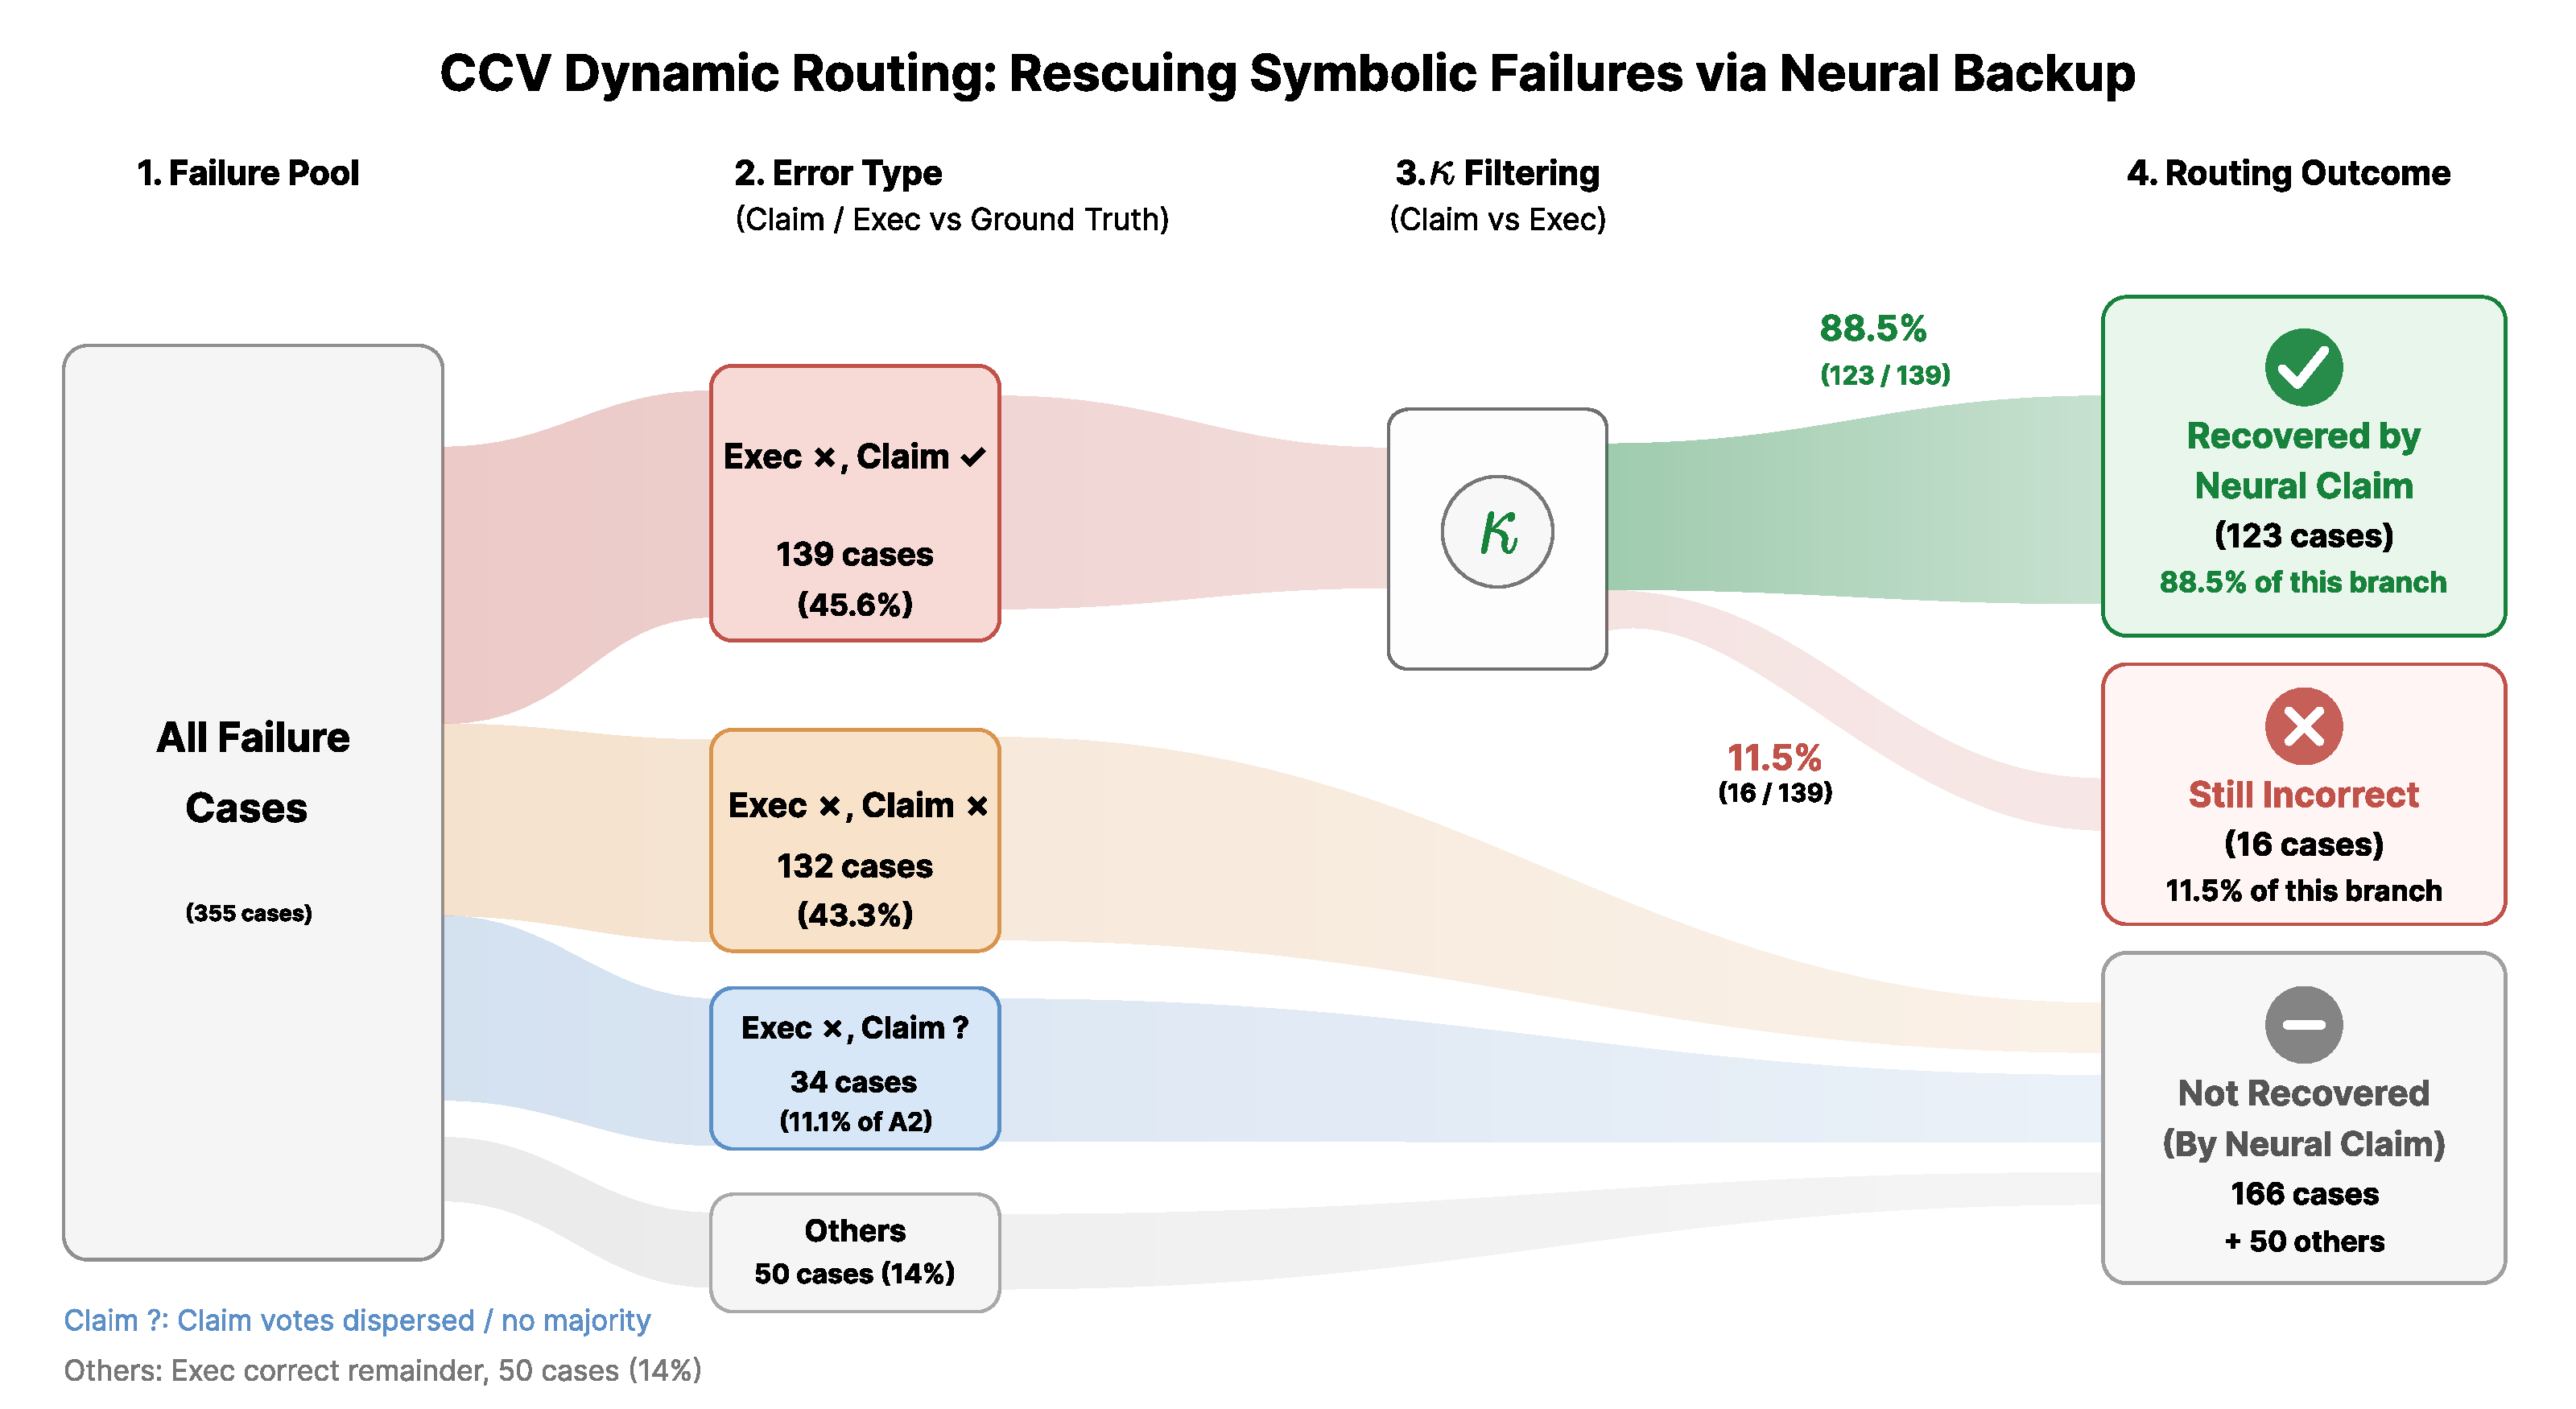
\includegraphics[width=\textwidth]{figures/figure4.pdf}
    \caption{\textbf{Error flow and dynamic routing.} Among \recheck{355} EAV failures with an oracle-correct candidate, wrong execution consensus dominates (\recheck{86\%}) and splits into three subtypes: Exec{\ding{55}}\,Claim{\ding{51}}, Exec{\ding{55}}\,Claim{\ding{55}}, and Exec{\ding{55}}\,Claim?. In the recoverable Exec{\ding{55}}\,Claim{\ding{51}} stream, the claim majority is correct while the execution majority is wrong; \ccv{}'s $\kappa$ filter routes \recheck{123/139} cases (\recheck{88.5\%}) to the correct neural-claim output, illustrating how output-pathway routing rescues samples when the symbolic channel collapses. This figure shows only the recovery direction; regressions are reported in Tables~\ref{tab:exchange-claim}--\ref{tab:regression-types}. Embedded counts await audit against those paired tables.}
    \label{fig:routing-sankey}
\end{figure*}

\section{Cross-Model Validation}
\label{app:cross-model}

Table~\ref{tab:cross-model} evaluates the same verification protocol on a lower-capacity Gemma4-E4B generator, using the same $\tau_{\text{exec}}{=}9$ as Qwen3.5-9B. The Gemma4 pool uses the same frozen $K{=}16$ protocol as Qwen: Geometry3K test (601), GeoQA test (754), and GPS-clean (146) form the three primary benchmarks, with GPS-full (208) reported for reference. The original overlapping aggregate contained \recheck{1,709} entries and \recheck{27,344} candidates; all aggregate results below await recomputation excluding GPS-full. The evaluation uses the standard benchmark files; it does not use the deprecated 400-question checkpoint-selection set.

\begin{table}[h]
\centering
\caption{Cross-model validation on the same frozen $K{=}16$ protocol for three primary benchmarks, with GPS-full excluded from the aggregate and reported for reference, using $\tau_{\text{exec}}{=}9$ for both models. Absolute accuracy differs because Qwen3.5-9B has higher model capacity than Gemma4-E4B, but the gain pattern is consistent: cross-layer $\kappa$ filtering and \ccv{} improve over surface consensus for both models with no additional model calls for verification on existing \sketch{} pools. Red values are the original aggregates pending recomputation; generator SFT and teacher-assisted reformatting costs are separate (Appendix~\ref{app:costs}).}
\label{tab:cross-model}
\small
\begin{tabular}{lcc}
\toprule
Method & Qwen3.5-9B & Gemma4-E4B \\
\midrule
Claim MV & \recheck{70.57} & \recheck{44.94} \\
Exec MV & \recheck{74.31} & \recheck{41.08} \\
EAV & \recheck{76.18} & \recheck{44.88} \\
PROVE-style $\kappa$ filter & \recheck{79.52} & \recheck{51.90} \\
\ccv{} (ours) & \recheck{\textbf{80.98}} & \recheck{\textbf{52.78}} \\
\midrule
\ccv{} $-$ Claim MV & \recheck{$+10.41$} & \recheck{$+7.84$} \\
\ccv{} $-$ EAV & \recheck{$+4.80$} & \recheck{$+7.90$} \\
Oracle & \recheck{93.27} & \recheck{91.75} \\
\bottomrule
\end{tabular}
\end{table}

The notable difference is that Gemma4 reverses the raw pathway ordering: Exec MV is below Claim MV (\recheck{41.08}\% vs \recheck{44.94}\%), whereas Qwen's execution pathway is stronger than its claim pathway. Consequently, EAV, an execution-first priority rule, is ineffective on Gemma4 (\recheck{44.88}\% vs \recheck{44.94}\% Claim MV). One possible explanation is weaker visual grounding: within-layer execution consensus is more easily dominated by correlated perception errors. The observed gain does not require execution to be the stronger raw channel. \ccv{} does not trust the raw execution vote; it uses claim--execution agreement as a precision filter. Even when the execution pathway is worse in aggregate, candidates where claim and execution agree remain informative, yielding $+\recheck{7.84}\pp$ over Claim MV and $+\recheck{7.90}\pp$ over EAV on Gemma4.

\section{Gemma4 $K$ Scaling}
\label{app:gemma-k-scaling}

Table~\ref{tab:gemma-k-scaling} repeats the $K$-scaling analysis on the frozen Gemma4-E4B $K{=}16$ pool by subsampling candidates; $K{<}16$ rows are averaged over four random subsamples. We keep $\tau_{\text{exec}}{=}9$ fixed to match the cross-model comparison in the main text.

\begin{table}[h]
\centering
\caption{Gemma4-E4B $K$ scaling from the frozen $K{=}16$ pool. Entries for $K{=}4,8$ are mean$\pm$std over four subsamples.}
\label{tab:gemma-k-scaling}
\small
\resizebox{\linewidth}{!}{
\begin{tabular}{rccccccc}
\toprule
$K$ & Claim MV & Exec MV & EAV & PROVE-style $\kappa$ & \ccv{} & Oracle & \ccv{} $-$ Claim MV \\
\midrule
4 & \recheck{$42.41{\pm}0.81$} & \recheck{$37.60{\pm}0.42$} & \recheck{$46.94{\pm}0.46$} & \recheck{$46.65{\pm}0.74$} & \recheck{$47.28{\pm}0.60$} & \recheck{$72.24{\pm}0.60$} & \recheck{$+4.87$} \\
8 & \recheck{$44.00{\pm}0.48$} & \recheck{$39.86{\pm}0.24$} & \recheck{$48.82{\pm}0.79$} & \recheck{$50.04{\pm}0.62$} & \recheck{$50.85{\pm}0.58$} & \recheck{$83.84{\pm}0.32$} & \recheck{$+6.85$} \\
16 & \recheck{44.94} & \recheck{41.08} & \recheck{44.88} & \recheck{51.90} & \recheck{52.78} & \recheck{91.75} & \recheck{$+7.84$} \\
\bottomrule
\end{tabular}
}
\end{table}

The Gemma4 gain increases with candidate budget, from $+\recheck{4.87}\pp$ at $K{=}4$ to $+\recheck{7.84}\pp$ at $K{=}16$, matching the qualitative scaling trend observed for Qwen.

\section{Gemma4 Implementation Details}
\label{app:gemma-implementation}

The Gemma4-E4B experiment uses the frozen checkpoint-720 LoRA adapter and the frozen rollout pool described in Appendix~\ref{app:cross-model}; no additional model calls are made for the verification comparisons. The adapter uses LoRA rank 8 and $\alpha=16$. On a 400-example format audit, the model reaches 96.0\% complete-section rate, 99.0\% VGF parse success, 96.0\% DSL syntax success, and 94.25\% DSL execution success, comparable to the format reliability of the Qwen model.

\section{$\kappa$ Matching Threshold Sensitivity}
\label{app:kappa-threshold}

The relation $X_i\approx Y_i$ is implemented by normalizing the claimed final answer and executed DSL answer, then applying numeric tolerance. Floating-point answers, fractions, square roots, and $\pi$ expressions are parsed to real values; degree symbols are treated as unit suffixes and removed before numeric comparison. For multiple-choice questions, numeric answers are first mapped to option letters using the fixed choice tolerance 0.02. Table~\ref{tab:kappa-threshold} reports an ablation that keeps the numeric absolute tolerance fixed at $10^{-3}$ and sweeps only the candidate-level relative tolerance used for $\kappa$.

\begin{table}[h]
\centering
\caption{Sensitivity to the candidate-level relative tolerance in $X_i\approx Y_i$ on the frozen Qwen3.5-9B s240 $K{=}16$, $T{=}0.8$ pool.}
\label{tab:kappa-threshold}
\small
\begin{tabular}{lccc}
\toprule
Setting & Candidate relative tolerance & \ccv{} accuracy & $\kappa$ candidates / precision \\
\midrule
$10^{-6}$ & 0.000001 & \recheck{80.98} & \recheck{15,535 / 87.07} \\
$10^{-4}$ & 0.0001 & \recheck{80.98} & \recheck{15,535 / 87.07} \\
$10^{-3}$ & 0.001 & \recheck{80.98} & \recheck{15,535 / 87.07} \\
default ($10^{-2}$) & 0.01 & \recheck{80.98} & \recheck{15,535 / 87.07} \\
$5{\times}10^{-2}$ & 0.05 & \recheck{80.98} & \recheck{15,535 / 87.07} \\
\bottomrule
\end{tabular}
\end{table}

All threshold settings yield identical results because geometry answers are effectively discrete: integers, simple fractions, radicals, angles, or multiple-choice letters. In this domain, claim--execution agreement is almost always binary: pairs either match exactly, or differ by margins much larger than even the loosest tolerance. This sweep supports stability over the tested relative tolerances on the original pool; the revised aggregate and other constants are audited separately (Appendix~\ref{app:constants}).

\section{Qualitative Case Studies}
\label{app:case-studies}

We present four representative cases from the frozen Qwen3.5-9B s240 $K{=}16$, $T{=}0.8$ pool, selected to illustrate the four behavioral modes of \ccv{}: (1)~successful rescue when execution consensus is wrong but claim is correct, (2)~hard cases where both pathways agree on a wrong answer, (3)~correlated perception errors that produce incorrect agreement, and (4)~fallback routing when no self-consistent candidate exists. Each case reports method outputs and the key DSL of the \ccv{}-selected candidate.

\subsection{CCV Rescue (Exec\ding{55}\,Claim\ding{51})}

\texttt{geometry3k\_test} qid~325. Expected: B (16). Choices: A=12, B=16, C=51, D=65.

\smallskip
\noindent \textbf{Method outputs.} Claim MV: B; Exec MV: C; EAV: C; \ccv{}: \textbf{B}.
\smallskip

\begin{minipage}{\linewidth}
\noindent \textbf{CCV-selected DSL} ($\kappa=1$, claim cluster 9, exec cluster 6):
\begin{verbatim}
angle_X = angle_L
x = angle_X / 4
answer = x          # 16.25 -> B
\end{verbatim}
\end{minipage}

\ccv{} selects a $\kappa$-consistent candidate whose claim and execution agree on B, while EAV follows a wrong execution majority (C). In this example the claim majority is correct and the execution majority is wrong, while the selected candidate agrees on the correct option.

\subsection{Hard Case: Exec\ding{55}\,Claim\ding{55}}

\texttt{geometry3k\_test} qid~72. Expected: A (3). Choices: A=3, B=4, C=6, D=7.

\smallskip
\noindent \textbf{Method outputs.} Claim MV: B; Exec MV: B; EAV: B; \ccv{}: B.
\smallskip

\begin{minipage}{\linewidth}
\noindent \textbf{CCV-selected DSL} ($\kappa=1$, claim cluster 15, exec cluster 15):
\begin{verbatim}
x = 4
answer = x          # 4.0 -> B
\end{verbatim}
\end{minipage}

All methods agree on the wrong answer. This case shows that cross-channel agreement can itself be wrong; agreement alone cannot establish correct premises.

\subsection{Correlated Perception Error}

\texttt{geometry3k\_test} qid~35. Expected: D (155). Choices: A=20, B=25, C=30, D=155.

\smallskip
\noindent \textbf{Method outputs.} Claim MV: B; Exec MV: B; EAV: B; \ccv{}: B.
\smallskip

\begin{minipage}{\linewidth}
\noindent \textbf{CCV-selected DSL} ($\kappa=1$, claim cluster 16, exec cluster 16):
\begin{verbatim}
arc_BC = 30
arc_AD = 20
angle_2 = (arc_BC + arc_AD) / 2
answer = angle_2    # 25.0 -> B
\end{verbatim}
\end{minipage}

This is a boundary case for \ccv{}: a correlated visual error makes both channels self-consistent around the wrong answer. With 16/16 candidates in both clusters, selection alone has no alternative evidence to break the incorrect consensus.

\subsection{Empty $\kappa$-Pool with Execution Fallback}

\texttt{geometry3k\_test} qid~56. Expected: C (70). Choices: A=66, B=68, C=70, D=72.

\smallskip
\noindent \textbf{Method outputs.} Claim MV: D; Exec MV: C; EAV: C; \ccv{}: \textbf{C}.
\smallskip

\begin{minipage}{\linewidth}
\noindent \textbf{CCV-selected DSL} ($\kappa=0$, claim cluster 10, exec cluster 16):
\begin{verbatim}
leg1 = 24
hypotenuse = 74
x = sqrt(hypotenuse**2 - leg1**2)
answer = x          # 70.0 -> C
\end{verbatim}
\end{minipage}

The $\kappa$-pool is empty (no candidate's claim matches its execution), so \ccv{} falls back to the execution-majority pathway. The large exec cluster (16/16) exceeds $\tau_{\text{exec}}$, providing the correct answer. This illustrates dual-pathway routing: when cross-channel agreement is absent, the deterministic symbolic path remains available as a fallback.

\section{Proofs for the Cross-Channel Verification Analysis}
\label{app:proofs}

\subsection{Definitions without an independence assumption}

Let $X_i$ be a normalized claim and $Y_i$ a normalized execution answer, allowing $Y_i=\bot$ for failure; $z^*$ denotes the ground-truth answer for the corresponding question. Let $E_i=\mathbf{1}[Y_i=z^*]$ and $C_i=\mathbf{1}[X_i=z^*]$. Agreement is $\kappa_i=\mathbf{1}[X_i=Y_i,\,Y_i\neq\bot]$. Failed executions count as incorrect and cannot agree. The precision identities hold for any joint distribution of $(X_i,Y_i)$, including the dependence created by generating the claim after the DSL source.

Within-channel correlation $\rho_e=\operatorname{Corr}(E_i,E_j)$ summarizes different candidates from the same question; $\rho_\kappa$ is its counterpart within retained candidate pairs. In contrast, the within-question $\phi$ coefficient correlates $C_i$ and $E_i$ across candidates of one question. We report its mean over questions where both binary variables have nonzero variance. These correlations measure different dependence relationships and cannot be substituted for one another.

\subsection{Precision identity and likelihood-ratio proof}

Theorem~\ref{thm:accuracy} follows by partitioning agreement into correct and incorrect execution: $P(\kappa=1)=t_\kappa+f_\kappa$. Bayes' rule gives $p_\kappa=t_\kappa/(t_\kappa+f_\kappa)$ whenever the denominator is positive.

For Proposition~\ref{prop:likelihood}, let $a=P(\kappa=1\mid E=1)$ and $b=P(\kappa=1\mid E=0)$. Since $0<p_e<1$ and $P(\kappa=1)>0$,
\begin{align}
 p_\kappa&=\frac{p_ea}{p_ea+(1-p_e)b},\\
 p_\kappa-p_e&=\frac{p_e(1-p_e)(a-b)}{p_ea+(1-p_e)b},\\
 p_\kappa>p_e&\Longleftrightarrow a>b.
\end{align}
For $b>0$, dividing the first expression by its complement yields Eq.~\eqref{eq:posterior-odds}. If $b=0$, positive retention implies $a>0$ and $p_\kappa=1$; if $a=b=0$, the retained pool is empty and its precision is undefined. No conditional-independence or wrong-answer-dispersion assumption is needed.

\begin{table}[h]
\centering
\caption{Agreement diagnostics on the original pools, all pending recomputation under the three-benchmark protocol. The pooled likelihood ratio is $a/b$; the question-stratified Mantel--Haenszel estimate excludes failed executions and is a separate association diagnostic, not the ratio used in the pooled odds identity. Pool-level CCV gains are measured separately.}
\label{tab:likelihood}
\small
\begin{tabular}{lcc}
\toprule
Metric & Qwen3.5-9B & Gemma4-E4B \\
\midrule
$P(\mathrm{agree}\mid\mathrm{exec}\ \checkmark)$ & \recheck{0.802} & \recheck{0.646} \\
$P(\mathrm{agree}\mid\mathrm{exec}\ \times)$ & \recheck{0.192} & \recheck{0.218} \\
Pooled likelihood ratio $a/b$ & \recheck{$4.18\times$} & \recheck{$2.96\times$} \\
Within-question Mantel--Haenszel (excluding $\bot$) & \recheck{$3.22\times$} & \recheck{$2.09\times$} \\
CCV relative to Claim MV & \recheck{$+10.41\pp$} & \recheck{$+7.84\pp$} \\
\bottomrule
\end{tabular}
\end{table}

Table~\ref{tab:likelihood} reports agreement enrichment for both model families. Before deployment on a new labeled pool, this comparison can reject settings with little expected precision benefit. Question-stratified diagnostics help distinguish within-question association from differences in question difficulty. Neither diagnostic establishes that the resulting selector will win a pool-level vote.

\subsection{SNR derivation and scope of Theorem~\ref{thm:snr}}

For $n$ exchangeable binary correctness indicators with common mean $p$ and pairwise correlation $\rho$,
\begin{equation}
 \operatorname{Var}\!\left(\frac{1}{n}\sum_{i=1}^n B_i\right)
 =\frac{p(1-p)}{n}\,[1+(n-1)\rho].
\end{equation}
Dividing $p-\tfrac12$ by the standard deviation gives the SNR in Theorem~\ref{thm:snr}. This variance identity is exact under the stated assumptions; using SNR to approximate majority reliability requires an additional distributional approximation and does not describe multiclass answer counts exactly.

For $p_e>\tfrac12$, nonempty fixed retained size $K_\kappa$, and positive variances, $\mathrm{SNR}_\kappa>\mathrm{SNR}_{\mathrm{raw}}$ is equivalent to
\begin{equation}
    \frac{p_\kappa-\tfrac{1}{2}}{p_e-\tfrac{1}{2}}
    >\sqrt{\frac{p_\kappa(1-p_\kappa)}{p_e(1-p_e)}
    \cdot\frac{K(1+(K_\kappa-1)\rho_\kappa)}{K_\kappa(1+(K-1)\rho_e)}}.
    \label{eq:snr_full_condition}
\end{equation}
When $p_e\leq\tfrac12$, compare the signed SNR expressions directly instead of dividing by $p_e-\tfrac12$; in particular, the displayed inequality cannot be applied unchanged to Gemma. Substituting a mean retained size for random $K_\kappa$ is another approximation. Candidate-level precision improvement alone does not establish this SNR comparison, and neither establishes a gain for CCV's weighted selection and fallback policy.

\subsection{Measured diagnostic illustration}
\label{app:numerical}

Table~\ref{tab:numerical-snr} preserves the original post-hoc Qwen statistics. Failed executions count as incorrect; within-channel correlations use ordered candidate pairs from the same question. The retained size is a mean, so these are descriptive SNR proxies rather than predicted selection accuracies.

\begin{table}[h]
\centering
\caption{Original statistics for the one-vs-rest SNR proxy, pending recomputation.}
\label{tab:numerical-snr}
\small
\begin{tabular}{lcccc}
\toprule
Method & $n$ & $p$ & $\rho$ & SNR \\
\midrule
Raw exec MV & 16 & \recheck{0.617} & \recheck{0.526} & \recheck{0.32} \\
$\kappa$-filtered MV & \recheck{9.09} & \recheck{0.871} & \recheck{0.646} & \recheck{1.33} \\
\bottomrule
\end{tabular}
\end{table}

The original retained pool is \recheck{23\%} more correlated while the SNR proxy improves by \recheck{$4.1\times$}. False agreement accounts for \recheck{12.9\%} of Qwen's retained candidates and \recheck{40.2\%} of Gemma's. Gemma's retained precision nevertheless rises from \recheck{33.4\%} to \recheck{59.8\%}: false agreement need not be negligible for the likelihood-ratio condition to hold. Pool-level improvements require separate empirical verification.

\section{Bidirectional Selection Analysis}
\label{app:regressions}

The exchange tables compare per-question correctness in both directions. Every count and derived win/loss ratio retains its reported value pending recomputation after excluding GPS-full. These paired tables and the older recovery-flow taxonomy must be reconciled during that audit; the recovery-only figure is not a substitute for net-change accounting.

\begin{table}[h]
\centering
\caption{Claim MV versus CCV correctness. Rows are Claim MV outcomes; columns are CCV outcomes. CCV records \recheck{237} wins and \recheck{59} losses (\recheck{4.02:1}).}
\label{tab:exchange-claim}
\small
\begin{tabular}{lcc}
\toprule
 & CCV correct & CCV incorrect \\
\midrule
Claim MV correct & \recheck{1,147} & \recheck{59} \\
Claim MV incorrect & \recheck{237} & \recheck{266} \\
\bottomrule
\end{tabular}
\end{table}

\begin{table}[h]
\centering
\caption{EAV versus CCV correctness. Rows are EAV outcomes; columns are CCV outcomes. CCV records \recheck{121} wins and \recheck{39} losses (\recheck{3.10:1}).}
\label{tab:exchange-eav}
\small
\begin{tabular}{lcc}
\toprule
 & CCV correct & CCV incorrect \\
\midrule
EAV correct & \recheck{1,263} & \recheck{39} \\
EAV incorrect & \recheck{121} & \recheck{286} \\
\bottomrule
\end{tabular}
\end{table}

\begin{table}[h]
\centering
\caption{Reported regression categories. The available taxonomy does not exhaustively account for the EAV losses; categories and totals await reconciliation rather than assigning an unsupported residual.}
\label{tab:regression-types}
\small
\begin{tabular}{lcc}
\toprule
Category & Against Claim MV & Against EAV \\
\midrule
False $\kappa$ agreement & \recheck{26/59} & \recheck{30/39} \\
Median wrong agreement-group size & \recheck{3} & \recheck{2} \\
Incorrect execution fallback & \recheck{33} & Not specified \\
Threshold effect & Not applicable & \recheck{7} \\
\bottomrule
\end{tabular}
\end{table}

In all \recheck{33} incorrect execution-fallback cases against Claim MV, no candidate executes to the correct answer; \recheck{15} exhibit unanimous 16/16 execution consensus. These failures show why a large fallback cluster cannot certify correct visual premises. The reported false-agreement losses often involve small retained groups, showing the separate risk of discarding a correct raw majority.

\section{Verification and Preparation Costs}
\label{app:costs}

Table~\ref{tab:costs} separates verification on an existing pool from the preparation needed to obtain it. CCV needs no additional model calls after SKETCH candidates have been generated, but the complete pipeline includes teacher reformatting and generator SFT. The entries below are the available cost observations, not a complete compute ledger for all experiments or teacher calls.

\begin{table}[h]
\centering
\caption{Available cost comparison. Pool-dependent totals are marked for recomputation. DSL execution is shared by execution-based selectors; external scorers incur separate model inference.}
\label{tab:costs}
\small
\begin{tabular}{lp{0.60\linewidth}}
\toprule
Component & Cost \\
\midrule
CCV aggregation & 2--4 ms/question on one CPU core; \recheck{4--7 s} for the original pool \\
DSL execution & $<$\recheck{10 s} for \recheck{27,344} candidates; shared with Exec MV, EAV, and PROVE-style filtering \\
SKETCH candidate length & Mean approximately \recheck{86} tokens \\
One-time LoRA SFT & Approximately 3.5 GPU-hours to the evaluated checkpoint; approximately 10.6 GPU-hours for the full run \\
URSA-RM weighted MV & One reward-model forward pass per candidate \\
CISC & One confidence self-assessment per candidate \\
Teacher reformatting & Required for generator preparation; complete compute accounting pending \\
\bottomrule
\end{tabular}
\end{table}

\section{Other Matching and Scoring Constants}
\label{app:constants}

Besides the development-selected execution threshold and the relative-tolerance sweep in Appendix~\ref{app:kappa-threshold}, the reported sensitivity checks cover absolute tolerance, answer-clustering tolerance, option mapping, and the claim-cluster weight. Absolute and clustering tolerance sweeps span four orders of magnitude with unchanged reported accuracy. The default option-mapping tolerance of 0.02 is not a local optimum, and claim weights in $[0,2]$ yield little variation. Table~\ref{tab:constants} records the available scope without inventing missing endpoints or accuracy values; those numeric results remain pending.

\begin{table}[h]
\centering
\caption{Sensitivity-table structure for the remaining constants. ``Pending'' denotes a numeric result absent from the supplied revision material, to be filled by the engineering audit. Red sweep results require recomputation.}
\label{tab:constants}
\small
\begin{tabular}{lp{0.32\linewidth}p{0.30\linewidth}}
\toprule
Constant & Available sweep scope & Reported result / numeric accuracy \\
\midrule
Absolute tolerance & Four orders of magnitude; endpoints pending & Unchanged / \recheck{pending} \\
Clustering tolerance & Four orders of magnitude; endpoints pending & Unchanged / \recheck{pending} \\
Option-mapping tolerance & Default 0.02; grid pending & Default not a local optimum / \recheck{pending} \\
Claim-cluster weight & $[0,2]$; default 0.5 & Small variation / \recheck{pending} \\
Agreement bonus & Common $+1$ in $\mathcal C_\kappa$ & No effect on argmax (exact) \\
\bottomrule
\end{tabular}
\end{table}

\paragraph{Why the $+1$ bonus is irrelevant to selection.}
For every $c_i\in\mathcal C_\kappa$, $\kappa_i=1$ and the score is $w_c|\mathrm{claim\_cluster}_i|+|\mathrm{exec\_cluster}_i|+1$. Removing the common constant preserves all score orderings and ties. When $\mathcal C_\kappa$ is empty, neither fallback branch uses this score. Thus the bonus cannot change the algorithm's output under a fixed tie-breaking rule.

\clearpage
\section{Notation}
\label{app:notation}

\begin{table}[h]
\centering
\caption{Notation for agreement, precision, dependence, and routing.}
\label{tab:notation}
\small
\begin{tabular}{lp{0.76\linewidth}}
\toprule
Symbol & Meaning \\
\midrule
$X_i,Y_i,z^*$ & Normalized neural claim, execution result, and correct answer \\
$\bot$ & Failed execution; counted as incorrect and excluded from agreement \\
$K,K_\kappa$ & Candidate count and retained agreement-pool size \\
$\kappa_i$ & Claim--execution agreement indicator, excluding $\bot$ \\
$\mathcal C_\kappa$ & Set of candidates with $\kappa_i=1$ \\
$t_\kappa,f_\kappa$ & Joint probabilities of agreement with correct and incorrect execution \\
$p_e,p_\kappa$ & Execution precision before and after agreement filtering \\
$a,b$ & Agreement probabilities conditional on correct and incorrect execution \\
$a/b$ & Agreement likelihood ratio in the posterior-odds identity \\
$\rho_e,\rho_\kappa$ & Execution-correctness correlation between within-question candidate pairs, before and after filtering \\
$\phi$ & Within-question correlation between claim and execution correctness across candidates \\
$\tau_{\mathrm{exec}}$ & Minimum execution-cluster size for execution fallback \\
$\mu_i$ & Cross-candidate, cross-layer agreement feature used in the learned ablation \\
$w_c$ & Claim-cluster weight, fixed to 0.5 in CCV \\
\bottomrule
\end{tabular}
\end{table}

\clearpage
\section*{NeurIPS Paper Checklist}


\begin{enumerate}

\item {\bf Claims}
    \item[] Question: Do the main claims made in the abstract and introduction accurately reflect the paper's contributions and scope?
    \item[] Answer: \answerYes{}.
    \item[] Justification: The abstract and introduction state the proposed cross-channel verification problem, the \ccv{} method, and the reported improvements. The scope is limited to verification over generated geometry candidates, with future extensions discussed in the conclusion.
    \item[] Guidelines:
    \begin{itemize}
        \item The answer \answerNA{} means that the abstract and introduction do not include the claims made in the paper.
        \item The abstract and/or introduction should clearly state the claims made, including the contributions made in the paper and important assumptions and limitations. A \answerNo{} or \answerNA{} answer to this question will not be perceived well by the reviewers. 
        \item The claims made should match theoretical and experimental results, and reflect how much the results can be expected to generalize to other settings. 
        \item It is fine to include aspirational goals as motivation as long as it is clear that these goals are not attained by the paper. 
    \end{itemize}

\item {\bf Limitations}
    \item[] Question: Does the paper discuss the limitations of the work performed by the authors?
    \item[] Answer: \answerYes{}.
    \item[] Justification: The conclusion discusses the present validation scope, including open-weight geometry models, proprietary frontier models, and independent premise verification as natural extensions.
    \item[] Guidelines:
    \begin{itemize}
        \item The answer \answerNA{} means that the paper has no limitation while the answer \answerNo{} means that the paper has limitations, but those are not discussed in the paper. 
        \item The authors are encouraged to create a separate ``Limitations'' section in their paper.
        \item The paper should point out any strong assumptions and how robust the results are to violations of these assumptions (e.g., independence assumptions, noiseless settings, model well-specification, asymptotic approximations only holding locally). The authors should reflect on how these assumptions might be violated in practice and what the implications would be.
        \item The authors should reflect on the scope of the claims made, e.g., if the approach was only tested on a few datasets or with a few runs. In general, empirical results often depend on implicit assumptions, which should be articulated.
        \item The authors should reflect on the factors that influence the performance of the approach. For example, a facial recognition algorithm may perform poorly when image resolution is low or images are taken in low lighting. Or a speech-to-text system might not be used reliably to provide closed captions for online lectures because it fails to handle technical jargon.
        \item The authors should discuss the computational efficiency of the proposed algorithms and how they scale with dataset size.
        \item If applicable, the authors should discuss possible limitations of their approach to address problems of privacy and fairness.
        \item While the authors might fear that complete honesty about limitations might be used by reviewers as grounds for rejection, a worse outcome might be that reviewers discover limitations that aren't acknowledged in the paper. The authors should use their best judgment and recognize that individual actions in favor of transparency play an important role in developing norms that preserve the integrity of the community. Reviewers will be specifically instructed to not penalize honesty concerning limitations.
    \end{itemize}

\item {\bf Theory assumptions and proofs}
    \item[] Question: For each theoretical result, does the paper provide the full set of assumptions and a complete (and correct) proof?
    \item[] Answer: \answerYes{}.
    \item[] Justification: Section~\ref{sec:method} states the latent-accuracy model and SNR condition, and Appendix~\ref{app:proofs} provides the corresponding proofs, assumptions, and numerical illustration.
    \item[] Guidelines:
    \begin{itemize}
        \item The answer \answerNA{} means that the paper does not include theoretical results. 
        \item All the theorems, formulas, and proofs in the paper should be numbered and cross-referenced.
        \item All assumptions should be clearly stated or referenced in the statement of any theorems.
        \item The proofs can either appear in the main paper or the supplemental material, but if they appear in the supplemental material, the authors are encouraged to provide a short proof sketch to provide intuition. 
        \item Inversely, any informal proof provided in the core of the paper should be complemented by formal proofs provided in appendix or supplemental material.
        \item Theorems and Lemmas that the proof relies upon should be properly referenced. 
    \end{itemize}

    \item {\bf Experimental result reproducibility}
    \item[] Question: Does the paper fully disclose all the information needed to reproduce the main experimental results of the paper to the extent that it affects the main claims and/or conclusions of the paper (regardless of whether the code and data are provided or not)?
    \item[] Answer: \answerYes{}.
    \item[] Justification: Sections~\ref{sec:method} and~\ref{sec:experiments}, together with Appendices~\ref{app:tau} and~\ref{app:diagnostics}, specify the output format, gating rule, benchmarks, rollout settings, threshold choice, and diagnostic protocol needed to reproduce the main comparisons.
    \item[] Guidelines:
    \begin{itemize}
        \item The answer \answerNA{} means that the paper does not include experiments.
        \item If the paper includes experiments, a \answerNo{} answer to this question will not be perceived well by the reviewers: Making the paper reproducible is important, regardless of whether the code and data are provided or not.
        \item If the contribution is a dataset and\slash or model, the authors should describe the steps taken to make their results reproducible or verifiable. 
        \item Depending on the contribution, reproducibility can be accomplished in various ways. For example, if the contribution is a novel architecture, describing the architecture fully might suffice, or if the contribution is a specific model and empirical evaluation, it may be necessary to either make it possible for others to replicate the model with the same dataset, or provide access to the model. In general. releasing code and data is often one good way to accomplish this, but reproducibility can also be provided via detailed instructions for how to replicate the results, access to a hosted model (e.g., in the case of a large language model), releasing of a model checkpoint, or other means that are appropriate to the research performed.
        \item While NeurIPS does not require releasing code, the conference does require all submissions to provide some reasonable avenue for reproducibility, which may depend on the nature of the contribution. For example
        \begin{enumerate}
            \item If the contribution is primarily a new algorithm, the paper should make it clear how to reproduce that algorithm.
            \item If the contribution is primarily a new model architecture, the paper should describe the architecture clearly and fully.
            \item If the contribution is a new model (e.g., a large language model), then there should either be a way to access this model for reproducing the results or a way to reproduce the model (e.g., with an open-source dataset or instructions for how to construct the dataset).
            \item We recognize that reproducibility may be tricky in some cases, in which case authors are welcome to describe the particular way they provide for reproducibility. In the case of closed-source models, it may be that access to the model is limited in some way (e.g., to registered users), but it should be possible for other researchers to have some path to reproducing or verifying the results.
        \end{enumerate}
    \end{itemize}


\item {\bf Open access to data and code}
    \item[] Question: Does the paper provide open access to the data and code, with sufficient instructions to faithfully reproduce the main experimental results, as described in supplemental material?
    \item[] Answer: \answerNo{}.
    \item[] Justification: Code is not publicly released at anonymous submission time. The experiments are based on offline selection over frozen candidate pools, and we plan to release evaluation and aggregation scripts upon acceptance, subject to institutional and dataset-license constraints.
    \item[] Guidelines:
    \begin{itemize}
        \item The answer \answerNA{} means that paper does not include experiments requiring code.
        \item Please see the NeurIPS code and data submission guidelines (\url{https://neurips.cc/public/guides/CodeSubmissionPolicy}) for more details.
        \item While we encourage the release of code and data, we understand that this might not be possible, so \answerNo{} is an acceptable answer. Papers cannot be rejected simply for not including code, unless this is central to the contribution (e.g., for a new open-source benchmark).
        \item The instructions should contain the exact command and environment needed to run to reproduce the results. See the NeurIPS code and data submission guidelines (\url{https://neurips.cc/public/guides/CodeSubmissionPolicy}) for more details.
        \item The authors should provide instructions on data access and preparation, including how to access the raw data, preprocessed data, intermediate data, and generated data, etc.
        \item The authors should provide scripts to reproduce all experimental results for the new proposed method and baselines. If only a subset of experiments are reproducible, they should state which ones are omitted from the script and why.
        \item At submission time, to preserve anonymity, the authors should release anonymized versions (if applicable).
        \item Providing as much information as possible in supplemental material (appended to the paper) is recommended, but including URLs to data and code is permitted.
    \end{itemize}


\item {\bf Experimental setting/details}
    \item[] Question: Does the paper specify all the training and test details (e.g., data splits, hyperparameters, how they were chosen, type of optimizer) necessary to understand the results?
    \item[] Answer: \answerYes{}.
    \item[] Justification: The setup describes the Geometry3K dev/test split, MathVerse OOD split, rollout count, decoding settings, $\tau$ selection, LoRA rank and scale, and frozen evaluation protocol. Implementation-level optimizer details should be included with the eventual code release.
    \item[] Guidelines:
    \begin{itemize}
        \item The answer \answerNA{} means that the paper does not include experiments.
        \item The experimental setting should be presented in the core of the paper to a level of detail that is necessary to appreciate the results and make sense of them.
        \item The full details can be provided either with the code, in appendix, or as supplemental material.
    \end{itemize}

\item {\bf Experiment statistical significance}
    \item[] Question: Does the paper report error bars suitably and correctly defined or other appropriate information about the statistical significance of the experiments?
    \item[] Answer: \answerYes{}.
    \item[] Justification: Section~\ref{sec:experiments} reports paired per-question significance tests for the main comparisons over the fixed 1,709-question evaluation set. We use paired bootstrap confidence intervals for accuracy differences and exact McNemar tests over discordant question outcomes; \ccv{} improves over Claim MV by $+10.42\pp$ (95\% CI $[8.48,12.40]\pp$, $p<10^{-12}$) and over EAV by $+4.80\pp$ (95\% CI $[3.39,6.26]\pp$, $p=5.7{\times}10^{-11}$).
    \item[] Guidelines:
    \begin{itemize}
        \item The answer \answerNA{} means that the paper does not include experiments.
        \item The authors should answer \answerYes{} if the results are accompanied by error bars, confidence intervals, or statistical significance tests, at least for the experiments that support the main claims of the paper.
        \item The factors of variability that the error bars are capturing should be clearly stated (for example, train/test split, initialization, random drawing of some parameter, or overall run with given experimental conditions).
        \item The method for calculating the error bars should be explained (closed form formula, call to a library function, bootstrap, etc.)
        \item The assumptions made should be given (e.g., Normally distributed errors).
        \item It should be clear whether the error bar is the standard deviation or the standard error of the mean.
        \item It is OK to report 1-sigma error bars, but one should state it. The authors should preferably report a 2-sigma error bar than state that they have a 96\% CI, if the hypothesis of Normality of errors is not verified.
        \item For asymmetric distributions, the authors should be careful not to show in tables or figures symmetric error bars that would yield results that are out of range (e.g., negative error rates).
        \item If error bars are reported in tables or plots, the authors should explain in the text how they were calculated and reference the corresponding figures or tables in the text.
    \end{itemize}

\item {\bf Experiments compute resources}
    \item[] Question: For each experiment, does the paper provide sufficient information on the computer resources (type of compute workers, memory, time of execution) needed to reproduce the experiments?
    \item[] Answer: \answerNo{}.
    \item[] Justification: We report the main training setup, checkpoint, candidate budget, and frozen evaluation pool size, but do not provide a complete accounting of wall-clock time and GPU-hours for all auxiliary scoring runs.
    \item[] Guidelines:
    \begin{itemize}
        \item The answer \answerNA{} means that the paper does not include experiments.
        \item The paper should indicate the type of compute workers CPU or GPU, internal cluster, or cloud provider, including relevant memory and storage.
        \item The paper should provide the amount of compute required for each of the individual experimental runs as well as estimate the total compute. 
        \item The paper should disclose whether the full research project required more compute than the experiments reported in the paper (e.g., preliminary or failed experiments that didn't make it into the paper). 
    \end{itemize}
    
\item {\bf Code of ethics}
    \item[] Question: Does the research conducted in the paper conform, in every respect, with the NeurIPS Code of Ethics \url{https://neurips.cc/public/EthicsGuidelines}?
    \item[] Answer: \answerYes{}.
    \item[] Justification: The work studies mathematical reasoning over public benchmark-style problems and model outputs, with no human-subject data collection, sensitive personal data, or safety-critical deployment.
    \item[] Guidelines:
    \begin{itemize}
        \item The answer \answerNA{} means that the authors have not reviewed the NeurIPS Code of Ethics.
        \item If the authors answer \answerNo, they should explain the special circumstances that require a deviation from the Code of Ethics.
        \item The authors should make sure to preserve anonymity (e.g., if there is a special consideration due to laws or regulations in their jurisdiction).
    \end{itemize}


\item {\bf Broader impacts}
    \item[] Question: Does the paper discuss both potential positive societal impacts and negative societal impacts of the work performed?
    \item[] Answer: \answerYes{}.
    \item[] Justification: The work is methodological and focuses on benchmark geometry reasoning. Potential benefits include more reliable and interpretable verification without additional inference, while potential risks arise if similar verification signals are over-trusted in high-stakes domains without domain-specific validation.
    \item[] Guidelines:
    \begin{itemize}
        \item The answer \answerNA{} means that there is no societal impact of the work performed.
        \item If the authors answer \answerNA{} or \answerNo, they should explain why their work has no societal impact or why the paper does not address societal impact.
        \item Examples of negative societal impacts include potential malicious or unintended uses (e.g., disinformation, generating fake profiles, surveillance), fairness considerations (e.g., deployment of technologies that could make decisions that unfairly impact specific groups), privacy considerations, and security considerations.
        \item The conference expects that many papers will be foundational research and not tied to particular applications, let alone deployments. However, if there is a direct path to any negative applications, the authors should point it out. For example, it is legitimate to point out that an improvement in the quality of generative models could be used to generate Deepfakes for disinformation. On the other hand, it is not needed to point out that a generic algorithm for optimizing neural networks could enable people to train models that generate Deepfakes faster.
        \item The authors should consider possible harms that could arise when the technology is being used as intended and functioning correctly, harms that could arise when the technology is being used as intended but gives incorrect results, and harms following from (intentional or unintentional) misuse of the technology.
        \item If there are negative societal impacts, the authors could also discuss possible mitigation strategies (e.g., gated release of models, providing defenses in addition to attacks, mechanisms for monitoring misuse, mechanisms to monitor how a system learns from feedback over time, improving the efficiency and accessibility of ML).
    \end{itemize}
    
\item {\bf Safeguards}
    \item[] Question: Does the paper describe safeguards that have been put in place for responsible release of data or models that have a high risk for misuse (e.g., pre-trained language models, image generators, or scraped datasets)?
    \item[] Answer: \answerNA{}.
    \item[] Justification: Not applicable. The system is evaluated on offline benchmark geometry reasoning and is not deployed in a user-facing or safety-critical setting.
    \item[] Guidelines:
    \begin{itemize}
        \item The answer \answerNA{} means that the paper poses no such risks.
        \item Released models that have a high risk for misuse or dual-use should be released with necessary safeguards to allow for controlled use of the model, for example by requiring that users adhere to usage guidelines or restrictions to access the model or implementing safety filters. 
        \item Datasets that have been scraped from the Internet could pose safety risks. The authors should describe how they avoided releasing unsafe images.
        \item We recognize that providing effective safeguards is challenging, and many papers do not require this, but we encourage authors to take this into account and make a best faith effort.
    \end{itemize}

\item {\bf Licenses for existing assets}
    \item[] Question: Are the creators or original owners of assets (e.g., code, data, models), used in the paper, properly credited and are the license and terms of use explicitly mentioned and properly respected?
    \item[] Answer: \answerNo{}.
    \item[] Justification: We cite the datasets and pretrained models used in the experiments and do not redistribute the original assets. A complete license table for all third-party assets is not included in the submission.
    \item[] Guidelines:
    \begin{itemize}
        \item The answer \answerNA{} means that the paper does not use existing assets.
        \item The authors should cite the original paper that produced the code package or dataset.
        \item The authors should state which version of the asset is used and, if possible, include a URL.
        \item The name of the license (e.g., CC-BY 4.0) should be included for each asset.
        \item For scraped data from a particular source (e.g., website), the copyright and terms of service of that source should be provided.
        \item If assets are released, the license, copyright information, and terms of use in the package should be provided. For popular datasets, \url{paperswithcode.com/datasets} has curated licenses for some datasets. Their licensing guide can help determine the license of a dataset.
        \item For existing datasets that are re-packaged, both the original license and the license of the derived asset (if it has changed) should be provided.
        \item If this information is not available online, the authors are encouraged to reach out to the asset's creators.
    \end{itemize}

\item {\bf New assets}
    \item[] Question: Are new assets introduced in the paper well documented and is the documentation provided alongside the assets?
    \item[] Answer: \answerNo{}.
    \item[] Justification: The paper does not introduce a newly released dataset at submission time. Experiments use existing public benchmarks and derived model outputs; we do not redistribute original benchmark images or questions, and any future release of derived metadata will respect the licenses of the source datasets.
    \item[] Guidelines:
    \begin{itemize}
        \item The answer \answerNA{} means that the paper does not release new assets.
        \item Researchers should communicate the details of the dataset\slash code\slash model as part of their submissions via structured templates. This includes details about training, license, limitations, etc. 
        \item The paper should discuss whether and how consent was obtained from people whose asset is used.
        \item At submission time, remember to anonymize your assets (if applicable). You can either create an anonymized URL or include an anonymized zip file.
    \end{itemize}

\item {\bf Crowdsourcing and research with human subjects}
    \item[] Question: For crowdsourcing experiments and research with human subjects, does the paper include the full text of instructions given to participants and screenshots, if applicable, as well as details about compensation (if any)? 
    \item[] Answer: \answerNA{}.
    \item[] Justification: The paper does not involve crowdsourcing experiments or research with human subjects.
    \item[] Guidelines:
    \begin{itemize}
        \item The answer \answerNA{} means that the paper does not involve crowdsourcing nor research with human subjects.
        \item Including this information in the supplemental material is fine, but if the main contribution of the paper involves human subjects, then as much detail as possible should be included in the main paper. 
        \item According to the NeurIPS Code of Ethics, workers involved in data collection, curation, or other labor should be paid at least the minimum wage in the country of the data collector. 
    \end{itemize}

\item {\bf Institutional review board (IRB) approvals or equivalent for research with human subjects}
    \item[] Question: Does the paper describe potential risks incurred by study participants, whether such risks were disclosed to the subjects, and whether Institutional Review Board (IRB) approvals (or an equivalent approval/review based on the requirements of your country or institution) were obtained?
    \item[] Answer: \answerNA{}.
    \item[] Justification: The paper does not involve crowdsourcing experiments or human-subject research, so IRB approval is not applicable.
    \item[] Guidelines:
    \begin{itemize}
        \item The answer \answerNA{} means that the paper does not involve crowdsourcing nor research with human subjects.
        \item Depending on the country in which research is conducted, IRB approval (or equivalent) may be required for any human subjects research. If you obtained IRB approval, you should clearly state this in the paper. 
        \item We recognize that the procedures for this may vary significantly between institutions and locations, and we expect authors to adhere to the NeurIPS Code of Ethics and the guidelines for their institution. 
        \item For initial submissions, do not include any information that would break anonymity (if applicable), such as the institution conducting the review.
    \end{itemize}

\item {\bf Declaration of LLM usage}
    \item[] Question: Does the paper describe the usage of LLMs if it is an important, original, or non-standard component of the core methods in this research? Note that if the LLM is used only for writing, editing, or formatting purposes and does \emph{not} impact the core methodology, scientific rigor, or originality of the research, declaration is not required.
    %this research? 
    \item[] Answer: \answerYes{}.
    \item[] Justification: The method and experiments describe the VLM generators, teacher-generated structured traces, and reformatting pipeline used to construct and evaluate \ccv{} candidates.
    \item[] Guidelines:
    \begin{itemize}
        \item The answer \answerNA{} means that the core method development in this research does not involve LLMs as any important, original, or non-standard components.
        \item Please refer to our LLM policy in the NeurIPS handbook for what should or should not be described.
    \end{itemize}

\end{enumerate}


\end{document}
